% !TeX program = xelatex
% ============================================================
%  CO3053 EMBEDDED SYSTEMS - ASSIGNMENT REPORT
%  Greenhouse micro-climate monitoring system (50 m x 50 m)
%  Compile with XeLaTeX (Overleaf: Menu -> Compiler -> XeLaTeX)
% ============================================================
\documentclass[11pt,a4paper]{report}

\usepackage{fontspec}
\setmainfont{Times New Roman}
\setsansfont{Arial}
\setmonofont{Consolas}

\usepackage[margin=2.5cm]{geometry}
\usepackage{setspace}\setstretch{1.25}
\usepackage{parskip}
\usepackage{amsmath,amssymb}
\usepackage{booktabs,tabularx,array,longtable,makecell,multirow}
\usepackage{enumitem}
\usepackage[table]{xcolor}
\usepackage{caption}
\usepackage{graphicx}
\usepackage[section]{placeins}
\usepackage{listings}
\usepackage{fancyhdr}
\usepackage[hidelinks]{hyperref}
\usepackage{tikz}
\usetikzlibrary{arrows.meta,positioning,shapes.geometric,shapes.misc,fit,calc,backgrounds,decorations.pathreplacing}
\usepackage{pgfplots}
\pgfplotsset{compat=1.16}

\pagestyle{fancy}
\fancyhf{}
\fancyhead[L]{\small CO3053 -- Embedded Systems}
\fancyhead[R]{\small Greenhouse Micro-climate Monitoring}
\fancyfoot[C]{\thepage}
\setlength{\headheight}{15pt}

\lstset{basicstyle=\ttfamily\small, frame=single, breaklines=true, columns=fullflexible,
        commentstyle=\itshape\color{gray}}

\tikzset{
  blk/.style={draw, rounded corners=3pt, align=center, minimum height=1cm, text width=3.6cm, font=\small},
  st/.style={draw, rounded corners=6pt, align=center, minimum height=0.9cm, minimum width=2.3cm, font=\small},
  arr/.style={-{Stealth[length=2.2mm]}, thick},
  lbl/.style={font=\footnotesize, fill=white, inner sep=1pt},
  proc/.style={draw, rectangle, align=center, text width=4.2cm, minimum height=0.8cm, font=\small},
  dec/.style={draw, diamond, aspect=2.2, align=center, inner sep=1pt, font=\small},
  term/.style={draw, rounded rectangle, align=center, minimum height=0.8cm, minimum width=2.2cm, font=\small},
  io/.style={draw, trapezium, trapezium left angle=70, trapezium right angle=110, align=center, minimum height=0.8cm, font=\small}
}

\newcolumntype{Y}{>{\raggedright\arraybackslash}X}
\newcommand{\todo}[1]{\textcolor{red}{[#1]}}
\definecolor{cA}{RGB}{31,119,180}
\definecolor{cB}{RGB}{214,96,39}
\newcommand{\tagA}{{\setlength{\fboxsep}{1pt}\colorbox{cA!15}{\textsf{\small A}}}}
\newcommand{\tagB}{{\setlength{\fboxsep}{1pt}\colorbox{cB!15}{\textsf{\small B}}}}
\newcommand{\tagAB}{{\setlength{\fboxsep}{1pt}\colorbox{gray!15}{\textsf{\scriptsize A+B}}}}
% "why this number" box
\newcommand{\why}[1]{\par\noindent\colorbox{gray!10}{\parbox{\dimexpr\linewidth-2\fboxsep}{\small\textbf{Where the numbers come from.} #1}}\par}

\begin{document}

% ---------------- TITLE PAGE ----------------
\begin{titlepage}
\begin{tikzpicture}[remember picture, overlay]
  % Outer Border
  \draw[line width = 2.5pt, color=blue!75!black] 
    ($(current page.north west) + (0.5in,-0.5in)$) 
    rectangle 
    ($(current page.south east) + (-0.5in,0.5in)$);
  % Inner Border
  \draw[line width = 0.8pt, color=blue!75!black] 
    ($(current page.north west) + (0.55in,-0.55in)$) 
    rectangle 
    ($(current page.south east) + (-0.55in,0.55in)$);
\end{tikzpicture}

\begin{center}
  {\large \textbf{VIETNAM NATIONAL UNIVERSITY -- HO CHI MINH CITY}}\\[0.2cm]
  {\large \textbf{HO CHI MINH CITY UNIVERSITY OF TECHNOLOGY}}\\[0.2cm]
  {\large \textbf{FACULTY OF COMPUTER SCIENCE AND ENGINEERING}}\\[0.7cm]

  
\includegraphics[width=3.6cm]{hcmut-logo.png}\\[0.6cm]

  {\large \textbf{CO3053 -- EMBEDDED SYSTEMS}}\\[0.25cm]
  \rule{0.86\textwidth}{0.8pt}\\[0.35cm]
  {\LARGE \textbf{ASSIGNMENT REPORT}}\\[0.3cm]
  {\Large \textbf{DESIGN OF A GREENHOUSE}}\\[0.15cm]
  {\Large \textbf{MICRO-CLIMATE MONITORING SYSTEM}}\\[0.15cm]
  {\normalsize \textit{System Architecture, Protocol Design, and Trade-off Analysis}}\\[0.25cm]
  \rule{0.86\textwidth}{0.8pt}\\[0.8cm]

  \renewcommand{\arraystretch}{1.3}
  \begin{tabular}{rll}
    \textbf{Course:}     & \multicolumn{2}{l}{CO3053 -- Embedded Systems} \\[0.12cm]
    \textbf{Topic:}      & \multicolumn{2}{l}{Greenhouse Micro-Climate Monitoring ($20\,\text{m}\times 50\,\text{m}$)} \\[0.12cm]
    \textbf{Class:}      & \multicolumn{2}{l}{CC01} \\[0.12cm]
    \textbf{Instructor:} & \multicolumn{2}{l}{Assoc. Prof. Phạm Hoàng Anh} \\[0.12cm]
    \textbf{Students:}   & \textbf{Nguyễn Quốc Thắng}     & \textbf{2353122} \\[0.12cm]
                         & \textbf{Võ Hoàng Nguyên}       & \textbf{2352844} \\[0.12cm]
                         & \textbf{Ngô Nguyễn Thành Nhân} & \textbf{2352849} \\
  \end{tabular}

  \vfill

  {\large \textbf{Ho Chi Minh City, September 2026}}
\end{center}
\end{titlepage}

\tableofcontents

% ============================================================
\chapter{Problem and Design Approach}\label{ch:intro}
% ============================================================

\section{Problem statement}
The task is to design a system that monitors air temperature, air humidity and light intensity inside a $20\times50$\,m greenhouse, and to discuss three criteria:
\begin{enumerate}[noitemsep]
  \item \textbf{Communication infrastructure} -- how measurements get from the sensors to a processing point (Chapter~\ref{ch:comm}).
  \item \textbf{Data correctness} -- how we make sure the values we act on are right (Chapter~\ref{ch:correct}).
  \item \textbf{Data analysis for alerts} -- how we decide when to warn the grower (Chapter~\ref{ch:alert}).
\end{enumerate}
At least two designs must be proposed and compared. We propose \textbf{Design A} (wired RS-485 bus) and \textbf{Design B} (wireless LoRa star). Both share the same sensing and the same alert software; they differ only in the communication layer, so the comparison is fair.

Two properties of the problem drive every decision:
\begin{itemize}
  \item \textbf{The climate is not uniform.} Areas near sunny walls, fans or misters differ from the centre, so one sensor cannot represent 1{,}000\,m\textsuperscript{2}. We need many measuring points and a way to combine them.
  \item \textbf{The physics is slow, the timing is soft.} Greenhouse air changes over minutes, not milliseconds. A delay of a few seconds causes no harm, so this is a \emph{soft} real-time system (Kopetz). What matters more is that alerts are \emph{trustworthy}: no false alarms, no missed events.
\end{itemize}

\section{Six families of design challenges and their priority}\label{sec:six}
Marwedel groups embedded design challenges into six families. They cannot all be optimised at once, so we ranked them for each design. When two goals conflict, the higher-ranked one wins.

\begin{table}[htbp]
\centering
\caption{Priority of the six challenge families (H = high, M = medium, L = low)}\label{tab:six}
\small
\begin{tabularx}{\textwidth}{>{\raggedright\arraybackslash}p{3.0cm} c c Y}
\toprule
\textbf{Challenge family} & \textbf{A} & \textbf{B} & \textbf{How it shows up here, and why A and B differ}\\
\midrule
1. Dependability & H (1st) & H (1st) & Drifting sensors, lost data, false alarms. Top for both: an alert system nobody trusts is useless.\\
2. Physical/cyber mismatch & H (2nd) & M (3rd) & A continuous temperature field is sampled at a few points; a hard threshold on noisy data flips on and off (a Zeno-like effect). B also delivers data with variable delay.\\
3. Resource efficiency & M (3rd) & H (2nd) & A is powered through the cable, so only cable cost matters. For B, an empty battery = a dead node, so \textbf{energy is part of dependability}.\\
4. Complexity & M & M--H & B must build its own channel access, time sync, buffering and encryption.\\
5. Societal impact & L & M & Alarm fatigue for growers (both); radio-band rules, battery waste and data security (B).\\
6. Data \& machine learning & L & L & Data volume is small; rules must be explainable to the grower. ML is left for future work.\\
\bottomrule
\end{tabularx}
\end{table}

The key consequence: in B, energy and latency pull in opposite directions (sending rarely saves battery but delays data). Instead of picking one fixed compromise, B uses \emph{adaptive reporting} (Section~\ref{sec:adaptive}).

\section{Shared architecture}\label{sec:arch}
\subsection{Four layers, hybrid processing, local gateway}
\begin{figure}[htbp]
\centering
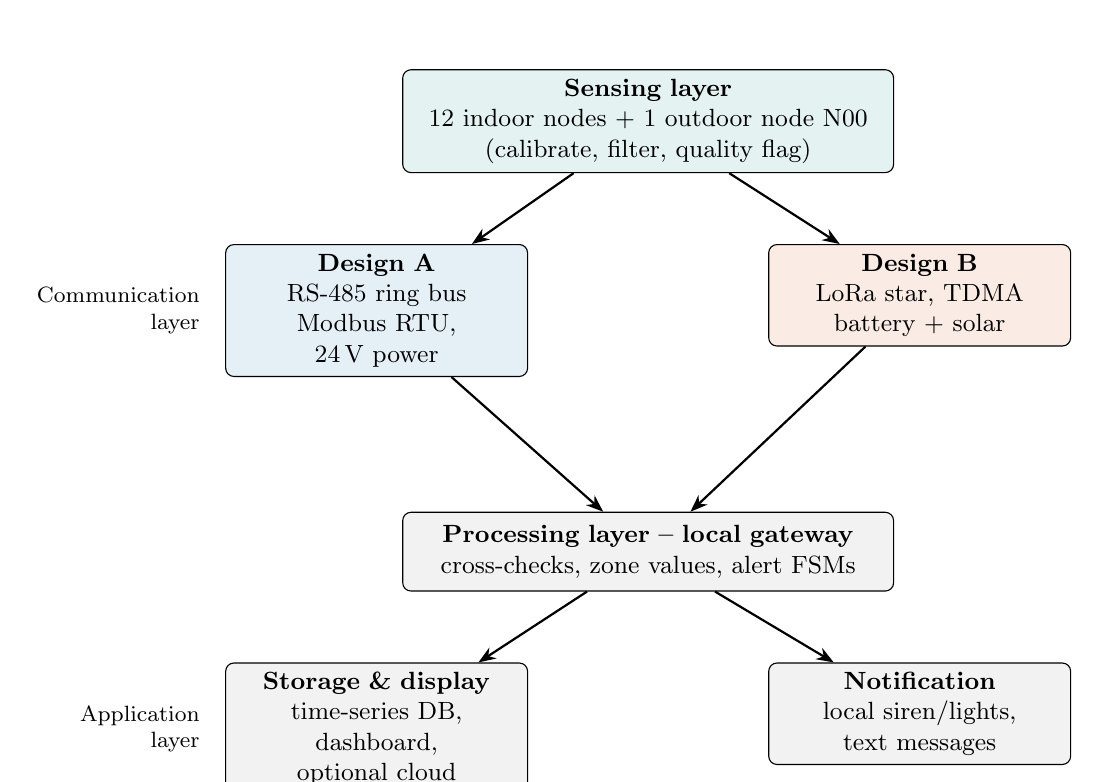
\begin{tikzpicture}[node distance=0.9cm and 0.6cm]
  \node[blk, text width=6cm, fill=teal!10] (n) {\textbf{Sensing layer}\\12 indoor nodes + 1 outdoor node N00\\(calibrate, filter, quality flag)};
  \node[blk, fill=cA!12, below left=0.9cm and -1.6cm of n] (a) {\textbf{Design A}\\RS-485 ring bus\\Modbus RTU, 24\,V power};
  \node[blk, fill=cB!12, below right=0.9cm and -1.6cm of n] (b) {\textbf{Design B}\\LoRa star, TDMA\\battery + solar};
  \node[blk, text width=6cm, fill=gray!10, below=4.3cm of n] (g) {\textbf{Processing layer -- local gateway}\\cross-checks, zone values, alert FSMs};
  \node[blk, fill=gray!10, below left=0.9cm and -1.6cm of g] (d) {\textbf{Storage \& display}\\time-series DB, dashboard,\\optional cloud};
  \node[blk, fill=gray!10, below right=0.9cm and -1.6cm of g] (w) {\textbf{Notification}\\local siren/lights,\\text messages};
  \draw[arr] (n) -- (a); \draw[arr] (n) -- (b);
  \draw[arr] (a) -- (g); \draw[arr] (b) -- (g);
  \draw[arr] (g) -- (d); \draw[arr] (g) -- (w);
  \node[font=\footnotesize, left=0.2cm of a, align=right] {Communication\\layer};
  \node[font=\footnotesize, left=0.2cm of d, align=right] {Application\\layer};
\end{tikzpicture}
\caption{Shared four-layer architecture; A and B differ only in the communication layer}\label{fig:arch}
\end{figure}

\begin{itemize}
  \item \textbf{Hybrid processing.} Each function runs where it has enough information to be done correctly. \emph{Nodes} do what needs raw samples: calibration, median filtering, range checks, quality flags -- so they send one clean value instead of five raw ones. The \emph{gateway} does what needs many nodes at once: detecting a drifting sensor by comparing neighbours, computing zone values, running the alert logic.
  \item \textbf{Local gateway, cloud optional.} All alert logic runs on a gateway inside the greenhouse, so the local siren still works when the Internet is down.
\end{itemize}

\subsection{Sensor placement}
\begin{figure}[htbp]
\centering
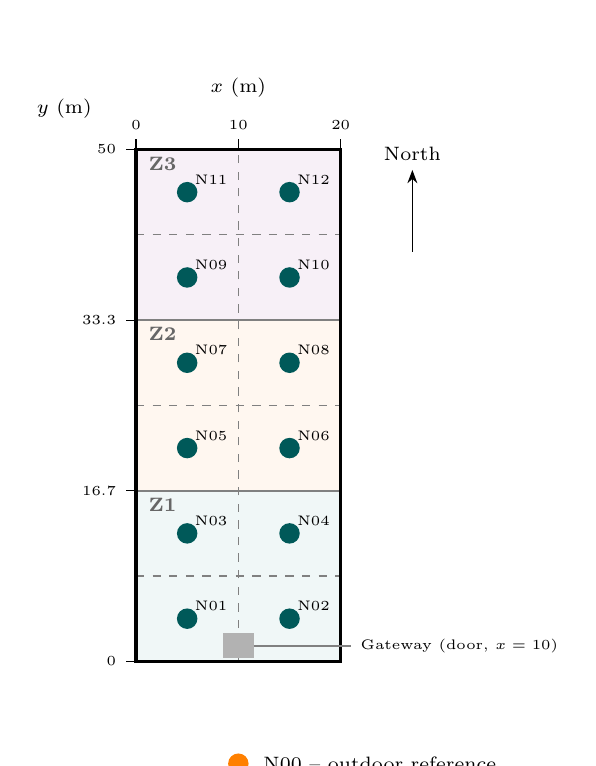
\begin{tikzpicture}[scale=0.13]
  \fill[teal!6] (0,0) rectangle (20,16.667);
  \fill[orange!6] (0,16.667) rectangle (20,33.333);
  \fill[violet!6] (0,33.333) rectangle (20,50);
  \draw[dashed,gray] (10,0) -- (10,50) (0,8.333) -- (20,8.333) (0,25) -- (20,25) (0,41.667) -- (20,41.667);
  \draw[thick,gray] (0,16.667) -- (20,16.667) (0,33.333) -- (20,33.333);
  \draw[very thick] (0,0) rectangle (20,50);
  \foreach \lbl/\y in {Z1/15.3, Z2/32, Z3/48.6}
    \node[font=\scriptsize\bfseries, gray!80!black] at (2.6,\y) {\lbl};
  \foreach \row/\y in {0/4.167,1/12.5,2/20.833,3/29.167,4/37.5,5/45.833}
    \foreach \col/\x in {1/5,2/15} {
      \pgfmathtruncatemacro{\id}{\row*2+\col}
      \fill[teal!70!black] (\x,\y) circle (1.0);
      \node[font=\tiny, above right=-1pt] at (\x,\y) {N\ifnum\id<10 0\fi\id};
    }
  \fill[gray!60] (8.5,0.3) rectangle (11.5,2.8);
  \node[font=\tiny, anchor=west] at (21,1.5) {Gateway (door, $x=10$)};
  \draw[gray] (11.5,1.5) -- (21,1.5);
  \fill[orange] (10,-10) circle (1.0);
  \node[font=\scriptsize, right] at (11.5,-10) {N00 -- outdoor reference};
  \foreach \v in {0,10,20} { \draw (\v,50) -- (\v,51); \node[font=\tiny, above] at (\v,51) {\v}; }
  \foreach \v/\t in {0/0,16.667/16.7,33.333/33.3,50/50} { \draw (0,\v) -- (-1,\v); \node[font=\tiny, left] at (-1,\v) {\t}; }
  \node[font=\scriptsize] at (10,56) {$x$ (m)};
  \node[font=\scriptsize] at (-7,54) {$y$ (m)};
  \draw[-{Stealth}] (27,40) -- (27,48); \node[font=\scriptsize, above] at (27,48) {North};
\end{tikzpicture}
\caption{12 nodes on a $2\times6$ grid, three zones Z1--Z3 of 4 nodes each, outdoor node N00 and the gateway at the door}\label{fig:layout}
\end{figure}

\why{We use a $2\times6$ grid (12 nodes); each node sits at the centre of a $10\times8.3$\,m cell, so no point of the greenhouse is more than $\sqrt{5^2+4.2^2}\approx 6.5$\,m from a node. The long axis is split into three $20\times16.7$\,m zones of exactly 4 nodes each. Four nodes per zone is the minimum that keeps a trustworthy zone median ($\geq 3$ good nodes, Section~\ref{sec:zone}) when one node fails. We evaluate alternative grid sizes ($N=6, 8, 10, 16, 20$) in Section~\ref{sec:nodesens}, confirming that 12 nodes offer the most balanced trade-off between coverage accuracy, zone fault tolerance, and network capacity. Nodes hang at crop-canopy height (default 1.5\,m, adjustable) inside a ventilated radiation shield. N00, outside the south wall, tells weather changes apart from problems inside the greenhouse.}

\subsection{Node hardware}
Both designs use \textbf{identical sensors}, so measurement error is not a difference between them: an SHT40 for temperature/humidity (factory-calibrated, has a built-in heater to clear condensation) and a TSL2591 for light (wide dynamic range, up to about 88\,klux). Midday light under the roof can come close to that limit, so the node reduces the sensor's gain and integration time automatically, and any reading at full scale is flagged SUSPECT instead of being trusted. The microcontroller, radio and power supply follow each design's priorities (Chapter~\ref{ch:comm}).

% ============================================================
\chapter{Criterion 1 -- Communication Infrastructure}\label{ch:comm}
% ============================================================

\section{What the infrastructure must provide}
Whatever the technology, the communication layer must deliver four things to the gateway:
\begin{enumerate}[noitemsep]
  \item \textbf{Completeness} -- every sample arrives eventually, even after a short outage (retry or backfill).
  \item \textbf{Timeliness} -- samples arrive fast enough for the alert logic (a few tens of seconds is fine; Chapter~\ref{ch:intro}).
  \item \textbf{Integrity and ordering} -- corrupted, duplicated or forged packets are detected; every sample has a timestamp.
  \item \textbf{No single point of failure in the network} -- one broken cable or one dead node must not blind a whole area.
\end{enumerate}
Design B has one extra requirement: \textbf{energy autonomy}, because its nodes run on batteries.

\section{Choosing the topology}
\begin{table}[htbp]
\centering
\caption{Candidate network topologies}\label{tab:topo}
\small
\begin{tabularx}{\textwidth}{>{\raggedright\arraybackslash}p{1.9cm} Y Y Y}
\toprule
\textbf{Topology} & \textbf{Strength} & \textbf{Weakness} & \textbf{Decision}\\
\midrule
Bus & Least cable; RS-485 is natively a multi-drop bus & A cable break cuts off every node behind it & \textbf{Design A}, upgraded to a \emph{ring bus} to remove the weakness\\
Star & Nodes fail independently & Wired: 12 separate cable runs; wireless: every node must be in range & \textbf{Design B}: the farthest node is about 46\,m from the gateway, well within one LoRa hop\\
Mesh & Redundant paths, long reach & Relay nodes must stay awake (drains batteries); routing; extra delay & Not needed at 50\,m\\
\bottomrule
\end{tabularx}
\end{table}

% ------------------------------------------------------------
\section{Design A: wired RS-485 ring bus with Modbus RTU}
% ------------------------------------------------------------
\subsection{Ring bus: surviving a cable break}
A normal bus loses every node beyond a cable break. The cable runs up the west column of nodes, across the north end and down the east column, so \textbf{both ends come back to the gateway}, which has two RS-485 ports, P1 and P2 (Figure~\ref{fig:ring}).
\begin{itemize}
  \item \textbf{Normal mode:} P1 is the Modbus master and polls all nodes. P2 only listens. Because P2 hears every frame on the cable, it acts as a \emph{continuity monitor}: if P2 stops hearing P1, the cable is broken somewhere.
  \item \textbf{Split mode (after a break):} P1 polls the nodes on its side, P2 polls the rest. \textbf{No node is lost.} The break lies between the last node answering P1 and the last node answering P2, so maintenance knows which cable segment to repair.
\end{itemize}

\begin{figure}[htbp]
\centering
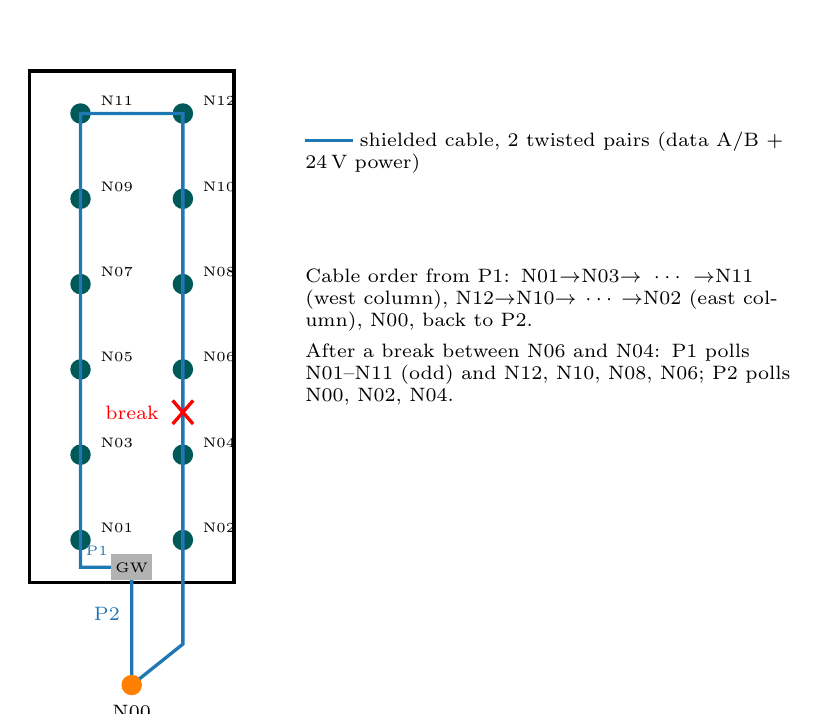
\begin{tikzpicture}[scale=0.13]
  \draw[very thick] (0,0) rectangle (20,50);
  \foreach \row/\y in {0/4.167,1/12.5,2/20.833,3/29.167,4/37.5,5/45.833}
    \foreach \col/\x in {1/5,2/15} {
      \pgfmathtruncatemacro{\id}{\row*2+\col}
      \fill[teal!70!black] (\x,\y) circle (1.0);
      \node[font=\tiny, anchor=west] at (\x+1,\y+1.2) {N\ifnum\id<10 0\fi\id};
    }
  \draw[cA, line width=1.2pt] (8,1.5) -- (5,1.5) -- (5,45.833) -- (15,45.833) -- (15,-6) -- (10,-10) -- (10,0.3);
  \fill[gray!60] (8,0.3) rectangle (12,2.8);
  \node[font=\tiny] at (10,1.5) {GW};
  \node[font=\tiny, cA, anchor=south] at (6.6,1.7) {P1};
  \node[font=\scriptsize, cA, anchor=east] at (9.8,-3) {P2};
  \fill[orange] (10,-10) circle (1.0); \node[font=\scriptsize, anchor=north] at (10,-11) {N00};
  \draw[red, very thick] (14,15.5) -- (16,17.8) (16,15.5) -- (14,17.8);
  \node[font=\scriptsize, red, anchor=east] at (13.6,16.6) {break};
  \node[font=\scriptsize, anchor=west, align=left, text width=6.2cm] at (26,42) {\textcolor{cA}{\rule[0.5ex]{6mm}{1.2pt}} shielded cable, 2 twisted pairs (data A/B + 24\,V power)};
  \node[font=\scriptsize, anchor=west, align=left, text width=6.2cm] at (26,24) {Cable order from P1: N01$\to$N03$\to\dots\to$N11 (west column), N12$\to$N10$\to\dots\to$N02 (east column), N00, back to P2.\\[3pt] After a break between N06 and N04: P1 polls N01--N11 (odd) and N12, N10, N08, N06; P2 polls N00, N02, N04.};
\end{tikzpicture}
\caption{Design A: RS-485 cable up one column and down the other, with both ends returning to the gateway}\label{fig:ring}
\end{figure}

\why{The cable is about 130\,m: two columns of about 45\,m each, 10\,m across the north end, and the loop out to N00 and back to the door. This is far below the 1{,}200\,m limit of RS-485, and 13 nodes plus 2 gateway transceivers stay well below the 32 standard loads a bus can drive.}

\subsection{Protocol: synchronised snapshot, then polling}
Every 30\,s the gateway:
\begin{enumerate}[noitemsep]
  \item broadcasts ``sample now'' with the current time -- all nodes measure at the same instant (one coherent spatial snapshot) and their clocks are synchronised for free;
  \item reads each node's registers (value, quality flags, sequence number, status) with a Modbus read request;
  \item retries once on a CRC error or timeout; if it still fails, marks that node MISSING for this cycle.
\end{enumerate}

\why{\emph{Why 30\,s?} A failed fan raises temperature by roughly 0.3--0.5\,°C per minute, so a 30\,s period gives about ten samples while the temperature climbs a few degrees -- enough for a reliable decision. \emph{Why 19{,}200\,bps?} At this speed one request/response takes about 26\,ms, so polling all 13 nodes takes about a third of a second: the bus is idle about 99\,\% of the time, leaving room for retries and backfill. A lower speed than the maximum is also more tolerant to electrical noise from pumps and fans.}

\subsection{Power and protection}
The second twisted pair carries 24\,V; each node has its own step-down converter. 24\,V is a safe extra-low voltage in a wet environment, and the voltage drop over 130\,m is small because each node draws only a few milliamperes. Each node has surge (TVS) protection; the gateway ports are galvanically isolated; enclosures are IP65 with waterproof cable glands.

% ------------------------------------------------------------
\section{Design B: wireless LoRa star with TDMA}
% ------------------------------------------------------------
\subsection{Radio link budget}
Before choosing radio settings we check that the farthest node can reach the gateway with margin to spare (Table~\ref{tab:link}).

\begin{table}[htbp]
\centering
\caption{Link budget to the farthest node (Design B)}\label{tab:link}
\small
\begin{tabular}{l r}
\toprule
\textbf{Item} & \textbf{Value}\\
\midrule
Transmit power & +14\,dBm\\
Antenna gain (transmitter + receiver) & +4\,dBi\\
Free-space path loss (46\,m at 923\,MHz) & $-65.0$\,dB\\
Assumed foliage and structural attenuation \cite{camapinto,itur} & $-25.0$\,dB\\
\textbf{Estimated received power} & $\mathbf{-72.0}$\,dBm\\
SX1276 sensitivity, SF7, 125\,kHz bandwidth & $-123$\,dBm\\
\textbf{Link margin} & \textbf{about 51\,dB}\\
\bottomrule
\end{tabular}
\end{table}

\why{
\textbf{+14\,dBm} is a standard output setting of the SX1276 radio (power at the chip, before the antenna; the legal check uses radiated power, see below).
\textbf{+4\,dBi}: a simple 2\,dBi whip antenna on each side.
\textbf{46\,m}: the farthest nodes (N11, N12 at the north end) are $\sqrt{5^2 + 45.8^2} \approx 46$\,m from the gateway at the south door.
\textbf{65.0\,dB} comes from the free-space formula $FSPL = 20\log_{10} d_{km} + 20\log_{10} f_{MHz} + 32.44$ with $d = 0.046$\,km and $f = 923$\,MHz.
\textbf{25.0\,dB excess loss (pessimistic assumption, not measured)}: estimated from published literature benchmarks (Cama-Pinto et al.\ \cite{camapinto} and ITU-R Recommendation P.833 \cite{itur}) rather than in-situ physical measurements in the target greenhouse. In dense humid vegetable canopies, specific wet foliage attenuation is estimated at $\alpha = 0.35$--$0.52$\,dB/m. Over an obstructed canopy propagation depth of $d_{\text{foliage}} \approx 35$\,m, foliage absorption accounts for $\approx 14$--$18$\,dB, with the remaining $7$--$11$\,dB assigned to multipath reflections from galvanized steel trusses and wet poly-film covering. This figure is intentionally chosen as a conservative safety buffer to evaluate worst-case connectivity.
\textbf{$-72.0$\,dBm} is the estimated received power under these heavy canopy assumptions.
\textbf{$-123$\,dBm} is the datasheet sensitivity at the fastest LoRa setting (SF7).
\textbf{Link margin $\approx 51$\,dB}: Even under an additional extreme fade allowance of 10--15\,dB during direct overhead spraying (pushing total excess loss to 35--40\,dB), the remaining $\approx 36$\,dB margin remains comfortably above standard commercial industrial safety benchmarks ($\ge 20$\,dB).
}

\textbf{Consequence.} Because the margin is large even under pessimistic assumptions, we use \textbf{SF7}, the fastest spreading factor. A packet then takes only about 67\,ms on air, which minimises both energy per packet and the chance of collisions. The gateway can also \emph{lower} each node's transmit power while keeping about 20\,dB margin -- too much margin is wasted battery.

\textbf{Regulatory check.} Legal limits apply to the power actually \emph{radiated}, not to the power at the chip. The node's radiated power is
\begin{equation}
  \text{EIRP} = P_{TX} + G_{antenna} = 14\ \text{dBm} + 2\ \text{dBi} = 16\ \text{dBm} \;(\approx 40\ \text{mW}),
\end{equation}
which equals about 13.9\,dBm ERP ($\approx 24$\,mW; ERP is EIRP minus 2.15\,dB). In Vietnam, LPWAN radios in the 920--923\,MHz band fall under QCVN~122:2020/BTTTT; before that regulation, LoRa devices had to use the generic short-range-device allocation limited to 25\,mW ERP. Our node stays within even this stricter limit, and in practice the power-control loop will run it lower. The same family of rules restricts channel occupancy by a \emph{duty-cycle} limit (commonly 1\,\%) or by \emph{listen-before-talk}. Our worst case -- dense mode, one 67\,ms packet every 30\,s -- is a duty cycle of 0.22\,\%. If listen-before-talk is required, the SX1276's channel-activity detection can check the channel at the start of each slot; this takes a few milliseconds and fits easily in the 1.5\,s slot. The exact limits must be confirmed against the current text of the regulation before deployment.

\subsection{Channel access: TDMA instead of random access}
If 13 nodes transmit at random times (pure ALOHA), two packets sometimes overlap and both are lost. With 13 nodes sending a 67\,ms packet every 60\,s, the standard ALOHA formula $P_{collision} = 1 - e^{-2G}$ (where $G$ is the fraction of time the channel is busy) gives about \textbf{3\,\%} lost packets -- each one costing a retransmission and battery. We therefore give each node its own time slot (Figure~\ref{fig:tdma}).

\begin{figure}[htbp]
\centering
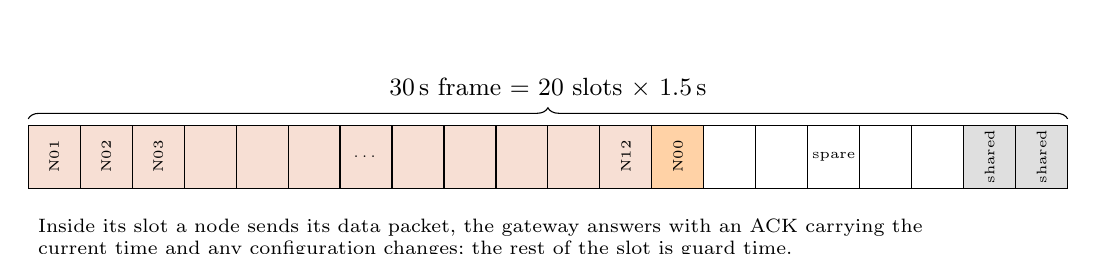
\begin{tikzpicture}[x=0.66cm, y=0.8cm]
  \foreach \i in {0,...,19} {
    \pgfmathsetmacro{\c}{\i<12 ? "cB!20" : (\i<13 ? "orange!35" : (\i<18 ? "white" : "gray!25"))}
    \draw[fill=\c] (\i,0) rectangle ++(1,1);
  }
  \foreach \i/\t in {0/N01,1/N02,2/N03,11/N12,12/N00} \node[font=\tiny, rotate=90] at (\i+0.5,0.5) {\t};
  \node[font=\tiny] at (6.5,0.5) {\dots};
  \node[font=\tiny] at (15.5,0.5) {spare};
  \node[font=\tiny, rotate=90] at (18.5,0.5) {shared};
  \node[font=\tiny, rotate=90] at (19.5,0.5) {shared};
  \draw[decorate, decoration={brace, amplitude=4pt}] (0,1.1) -- (20,1.1) node[midway, above=4pt, font=\small] {30\,s frame = 20 slots $\times$ 1.5\,s};
  \node[font=\scriptsize, anchor=west, align=left, text width=11.5cm] at (0,-0.8) {Inside its slot a node sends its data packet, the gateway answers with an ACK carrying the current time and any configuration changes; the rest of the slot is guard time.};
\end{tikzpicture}
\caption{TDMA frame of Design B}\label{fig:tdma}
\end{figure}

\why{The frame is 30\,s because that is the sampling period (same as Design A). 20 slots give 12 indoor nodes + N00 + 5 spare slots for extra nodes + 2 shared slots for urgent packets. Each slot is 1.5\,s, while a data packet (about 67\,ms) plus ACK (about 41\,ms) needs roughly 0.1\,s, so there is a large guard time. That guard time matters: a node's crystal clock drifts only a few milliseconds between two ACKs, and every ACK re-synchronises it, so nodes never slide into a neighbour's slot and no separate beacon is needed.}

\subsection{Reliable delivery}
Radio packets can still be lost (interference, a person standing next to the antenna). Each packet is acknowledged; if no ACK comes back, the node retries up to three times, and if that fails the data stays in a \textbf{24-hour store-and-forward buffer} and is sent with the next packet. The gateway reorders by timestamp and drops duplicates using sequence numbers. Data may arrive late, but it is not lost.

\subsection{Adaptive reporting: saving energy without delaying alerts}\label{sec:adaptive}
The node \emph{samples} every 30\,s (sensors cost very little energy), but \emph{transmits} adaptively -- because the radio is by far the largest energy consumer:
\begin{itemize}[noitemsep]
  \item \textbf{Sparse mode:} while values are far from any alert threshold, send one packet every 120\,s containing the last four samples.
  \item \textbf{Dense mode:} when a value is close to an alert threshold (e.g.\ within 1\,°C of the warning level) or changes quickly, send every sample.
  \item \textbf{Urgent:} a sensor fault is sent immediately in a shared slot.
\end{itemize}
The gateway pushes the ``close to threshold'' levels down to the nodes inside ACKs. Nodes never decide on alerts; they only decide \emph{when to talk}. The simulation in Chapter~\ref{ch:pe} compares this policy with the only fixed schedule that has the same freshness -- sending every sample (every 30\,s): alert delay is the same, while the number of transmissions falls by more than half.

\subsection{Energy}
Each node runs on a LiFePO\textsubscript{4} 18650 cell (chosen because it tolerates greenhouse heat better than ordinary Li-ion) and a small solar panel. Between measurements the microcontroller sleeps, the radio is off and the light sensor is powered down. Once the radio is duty-cycled this aggressively, node consumption becomes comparable to battery self-discharge. A small solar panel easily covers daily needs even under shaded roofs, requiring the battery only for cloudy intervals.

\subsection{Security}
Unlike a cable, a radio channel can be overheard or spoofed. Each node has its own AES-128 key; packets are encrypted and carry a short integrity code, and the gateway rejects any packet whose frame counter does not increase (anti-replay).

% ------------------------------------------------------------
\clearpage
\section{Summary of the two infrastructures}
Table~\ref{tab:infra} summarizes how the wired RS-485 ring and the wireless LoRa star realize each key communication objective. While Design A delivers deterministic polling and zero battery maintenance through physical cabling, Design B provides modular, cable-free installation and resilient store-and-forward buffering to ride through temporary radio fades.

\begin{table}[htbp]
\centering
\caption{How each design meets the infrastructure requirements}\label{tab:infra}
\small
\renewcommand{\arraystretch}{0.95}
\begin{tabularx}{\textwidth}{>{\raggedright\arraybackslash}p{2.8cm} Y Y}
\toprule
\textbf{Requirement} & \textbf{Design A (RS-485 ring)} & \textbf{Design B (LoRa star)}\\
\midrule
Completeness & Retry once per cycle; gateway reads node buffers after a restart & ACK, 3 retries, 24\,h buffer\\
Timeliness & Fixed, under one cycle & Variable (up to the report period); near-threshold data sent immediately\\
Integrity, order & Modbus CRC; timestamps from synchronised broadcast & Radio CRC + integrity code; sequence numbers; clock sync via ACK\\
Single failures & One cable break: no node lost & Failures are independent per node\\
Energy & Not an issue (24\,V over cable) & Sleep, SF7, adaptive reporting, solar\\
Security & Physical access needed & Encryption, integrity code, anti-replay\\
Main cost & 150\,m STP cable, PVC conduit, and wiring labor (\$635 CAPEX) & Solar/battery hardware and Year-3 cell renewal (\$491 CAPEX)\\
\bottomrule
\end{tabularx}
\end{table}

\textbf{Takeaway.} For permanent commercial installations with fixed gutter layouts, Design A's upfront cabling investment is justified by predictable polling latency. For flexible vegetable greenhouses where bed geometry changes seasonally, Design B's wireless autonomy and adaptive reporting provide superior practical agility.

% ============================================================
\chapter{Criterion 2 -- Data Correctness}\label{ch:correct}
% ============================================================

\section{Where errors come from}
A value can go wrong anywhere along its path: \emph{sensor $\to$ node $\to$ link $\to$ gateway}. No single technique catches every error, so we use three layers, each aimed at a different kind of error (Table~\ref{tab:layers}). The first two layers are identical in A and B; the third differs only in how transmission errors are handled.

\begin{table}[htbp]
\centering
\caption{Three layers of data correctness}\label{tab:layers}
\small
\begin{tabularx}{\textwidth}{>{\raggedright\arraybackslash}p{2.3cm} Y Y Y}
\toprule
\textbf{Layer} & \textbf{Error type} & \textbf{Countermeasure} & \textbf{A vs B}\\
\midrule
Sensor & Systematic offset, sun heating the sensor, condensation, poor placement & Good sensors, radiation shield, 2-point calibration, heater & Same\\
Node & Random noise, electrical spikes, impossible values & Repeated reads, median, range and rate checks, quality flag & Same\\
Gateway & Drifting / stuck / dead sensors; lost, corrupted, late or forged packets & Neighbour comparison, zone median, sequence numbers, timestamps & A: CRC + retry. B: CRC + integrity code, ACK, buffer, \emph{late-data handling}\\
\bottomrule
\end{tabularx}
\end{table}

\section{Sensor layer: prevent errors at the source}
\begin{itemize}
  \item \textbf{Radiation shield.} Direct sun on a bare temperature sensor makes it read several degrees above the real air temperature -- the largest single error source in a greenhouse. A ventilated multi-plate shield removes it.
  \item \textbf{Placement.} At canopy height, away from misting nozzles, fans and glass walls; light sensor on top of the mast, facing up.
  \item \textbf{Two-point calibration.} Before installation each sensor is compared with a reference at two temperatures; the correction $x_{true} = a\,x_{measured} + b$ is stored in the node and repeated periodically.
  \item \textbf{Condensation.} After misting, water on the humidity sensor makes it stick near 100\,\%RH. The SHT40's built-in heater is switched on briefly to dry it; readings during recovery are flagged SUSPECT.
  \item \textbf{Light saturation.} The TSL2591 tops out at about 88\,klux. Outdoor sun exceeds this, so N00 looks through a diffuser of known attenuation. Indoor midday light can also come close to the limit (roof transmission is often 60--80\,\% of outdoor light), so indoor nodes reduce gain and integration time automatically, and a reading at full scale is flagged SUSPECT; if this happens often, a diffuser is added to the indoor sensors too.
\end{itemize}

\section{Node layer: clean every sample}
Every cycle, each node runs the procedure of Figure~\ref{fig:filter} and attaches a quality flag to the value.

\begin{figure}[htbp]
\centering
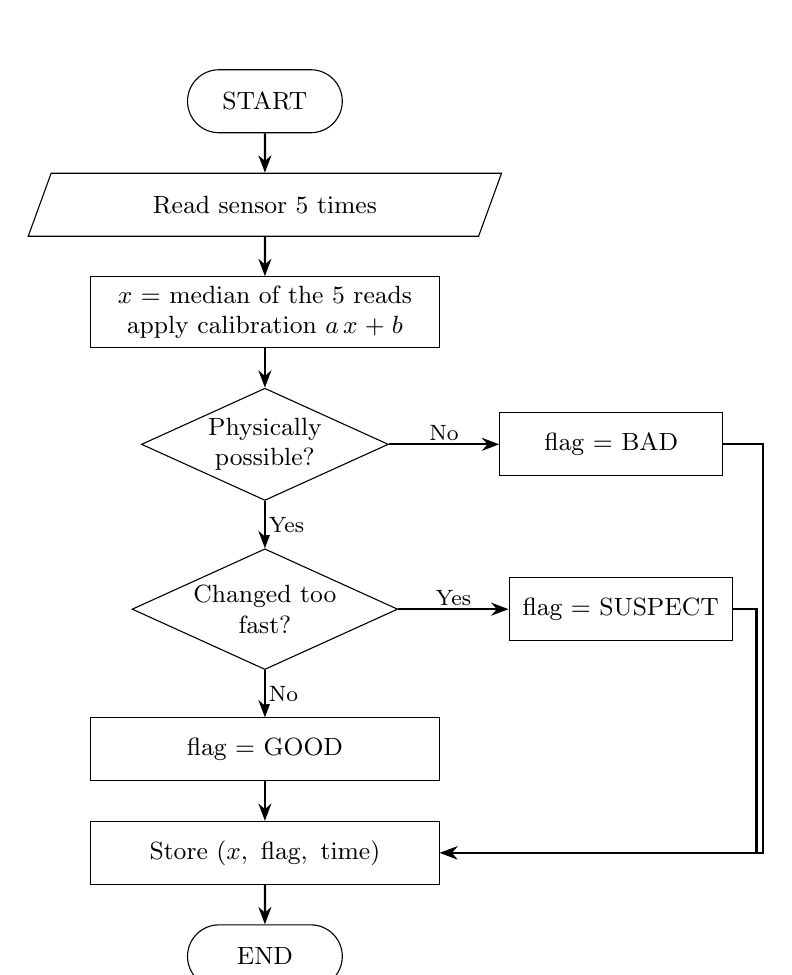
\begin{tikzpicture}[node distance=0.5cm]
  \node[term] (s) {START};
  \node[io, below=of s] (r) {Read sensor 5 times};
  \node[proc, below=of r] (m) {$x$ = median of the 5 reads\\apply calibration $a\,x + b$};
  \node[dec, below=of m] (d1) {Physically\\possible?};
  \node[proc, right=1.4cm of d1, text width=2.6cm] (bad) {flag = BAD};
  \node[dec, below=0.6cm of d1] (d2) {Changed too\\fast?};
  \node[proc, right=1.4cm of d2, text width=2.6cm] (sus) {flag = SUSPECT};
  \node[proc, below=0.6cm of d2] (ok) {flag = GOOD};
  \node[proc, below=of ok] (pk) {Store $(x,\ \text{flag},\ \text{time})$};
  \node[term, below=of pk] (e) {END};
  \draw[arr] (s) -- (r); \draw[arr] (r) -- (m); \draw[arr] (m) -- (d1);
  \draw[arr] (d1) -- node[lbl, above]{No} (bad);
  \draw[arr] (d1) -- node[lbl, right]{Yes} (d2);
  \draw[arr] (d2) -- node[lbl, above]{Yes} (sus);
  \draw[arr] (d2) -- node[lbl, right]{No} (ok);
  \draw[arr] (ok) -- (pk); \draw[arr] (pk) -- (e);
  \draw[arr] (bad.east) -- ++(0.5,0) |- (pk.east);
  \draw[arr] (sus.east) -- ++(0.3,0) |- (pk.east);
\end{tikzpicture}
\caption{Filtering and validation on every node (both designs)}\label{fig:filter}
\end{figure}

\why{\emph{Five reads, median:} five reads take only about 50\,ms. The median of five ignores up to two corrupted reads, whereas an average would be dragged by a single spike. \emph{Physically possible:} temperature 0--60\,°C, humidity 0--100\,\%, light not negative -- anything else is a hardware fault. \emph{Too fast:} a change of more than 3\,°C per minute. Real greenhouse air has too much thermal inertia to change that fast, so such a jump is almost certainly a glitch; it is flagged, not deleted, in case it is real.}

Only \textbf{GOOD} values may trigger or clear environmental alerts. SUSPECT values are still displayed (marked), BAD values are not.

We deliberately do \emph{not} put a smoothing filter (moving average) on the alert path: it would delay the alert by about a minute, and the alert logic already rejects short disturbances on its own (Chapter~\ref{ch:alert}). Smoothing is applied only to dashboard curves.

\section{Gateway layer: catch what a single node cannot see}
A node cannot know that it is drifting -- its readings look perfectly plausible. Only a comparison with other nodes reveals it. This is why fault detection runs on the gateway.

\subsection{Detecting faulty sensors}
\begin{itemize}
  \item \textbf{Drift.} For each node, compute the difference between its value and the median of its grid neighbours. If the difference stays above 2\,°C for 30 minutes while the neighbours agree with each other, the node is marked as drifting and removed from calculations; maintenance is notified.
  \item \textbf{Stuck value.} A node whose reading has not changed at all for 30 minutes while all other nodes are changing is marked BAD.
  \item \textbf{Dead node.} No data for three expected deliveries: three polls in A (1.5\,min), three report periods in B (6\,min). B detects a dead node more slowly -- one of its costs.
\end{itemize}

\why{\emph{2\,°C:} normal differences between neighbouring nodes (sunny side vs.\ shaded side) are around 1\,°C, and each sensor is accurate to about $\pm0.2$\,°C, so 2\,°C is clearly abnormal without triggering on normal gradients. \emph{30 minutes:} a local event (a door opened, a heater near one node) passes within minutes; a drift does not. Requiring persistence avoids blaming a healthy node for a real local event.}

\subsection{Zone value: tolerate one bad node per zone}\label{sec:zone}
Alerts are never based on a single node. For each zone we compute the median of its GOOD nodes and classify the result by how many GOOD nodes there are:

\begin{table}[htbp]
\centering
\caption{Zone validity}\label{tab:zonevalid}
\small
\begin{tabularx}{\textwidth}{>{\raggedright\arraybackslash}p{2.4cm} >{\raggedright\arraybackslash}p{2.6cm} Y}
\toprule
\textbf{GOOD nodes} & \textbf{Zone status} & \textbf{Zone value and use}\\
\midrule
4 or 3 & VALID & Median of the GOOD nodes; used for alerts. One wrong value cannot move a median of 3 or 4 values.\\
2 & DEGRADED & The ``median'' of two values is just their average, so one bad node \emph{could} pull it. Used for alerts only if the two nodes agree within 1\,°C; otherwise treated as invalid. A device alert ``zone degraded'' is raised in both cases.\\
0 or 1 & INVALID & No zone value; the zone's alert FSMs go to SENSOR\_FAULT.\\
\bottomrule
\end{tabularx}
\end{table}

So, \textbf{as long as a zone is VALID, even a faulty node that has not yet been detected cannot cause a false alarm}. In the DEGRADED state protection is weaker, which is why it requires agreement and is reported for maintenance. An INVALID zone is \emph{never} silently treated as normal.

\why{\emph{1\,°C:} two healthy nodes in the same zone normally differ by less than about 1\,°C (sunny vs.\ shaded side), so a larger disagreement means one of them cannot be trusted and we cannot tell which.}

This argument assumes nodes fail independently. That holds for B (separate radio links) but not for a plain bus in A, where one cable break takes out many nodes together -- which is exactly why Design A uses the ring bus.

\subsection{Real event or faulty sensor?}
\begin{table}[htbp]
\centering
\caption{Telling a real event from a sensor fault}\label{tab:realfault}
\small
\begin{tabularx}{\textwidth}{>{\raggedright\arraybackslash}p{2.6cm} Y Y}
\toprule
\textbf{Clue} & \textbf{Real event} & \textbf{Sensor fault}\\
\midrule
Space & Several neighbouring nodes move together & One node deviates alone\\
Speed & Consistent with thermal inertia (minutes) & Sudden jump, or no change at all\\
Cause & Explained by sun, outdoor node N00, a stopped fan & No link with sun, N00 or other nodes\\
Time & Follows day/night, recovers when the cause ends & Persists, never recovers\\
\bottomrule
\end{tabularx}
\end{table}

The hard case is a \emph{real} hot spot affecting only one node (e.g.\ a fan next to it failed). The zone median ignores it, but the separate ``uneven temperature'' alert (Section~\ref{sec:derived}) still catches it.

\subsection{Missing data vs.\ late data}
This is where A and B differ most. In A, a value not received in its polling cycle really is missing. In B, a value may simply not have been \emph{sent yet} (sparse mode sends every 120\,s). If the gateway treated ``not yet arrived'' as ``missing'', it would constantly declare sensor faults. We therefore use one extra quality level:

\begin{table}[htbp]
\centering
\caption{Quality levels and how they are used}\label{tab:quality}
\small
\begin{tabularx}{\textwidth}{l Y c}
\toprule
\textbf{Level} & \textbf{Meaning} & \textbf{Used for alerts}\\
\midrule
GOOD & Passed all checks & Yes\\
SUSPECT & Changed too fast, or node suspected of drift & No\\
BAD & Impossible value, stuck, sensor error & No\\
PENDING (B only) & Not received yet, but still within the expected delivery delay & No, and \emph{not penalised}\\
MISSING & Not received after the expected delivery delay & No\\
\bottomrule
\end{tabularx}
\end{table}

Two further rules: missing values are \textbf{never interpolated for alerts} (an estimate is not a measurement; interpolation is used only to draw heat maps, labelled ``estimated''), and every data gap is logged with its cause (packet loss, node fault, cable fault).

\clearpage
\section{Error scenarios at a glance}
Table~\ref{tab:fail} maps each potential error condition across the sensing, communication, and processing layers to its corresponding detection mechanism and defensive response in Design A and Design B.

\begin{table}[htbp]
\centering
\caption{Main error scenarios and how they are handled}\label{tab:fail}
\small
\renewcommand{\arraystretch}{0.95}
\begin{tabularx}{\textwidth}{>{\raggedright\arraybackslash}p{0.8cm} >{\raggedright\arraybackslash}p{3.8cm} >{\raggedright\arraybackslash}p{3.6cm} Y}
\toprule
& \textbf{Scenario} & \textbf{Detected by} & \textbf{Handling}\\
\midrule
\tagAB & Electrical spike & Median, rate check & Spike discarded\\
\tagAB & Sun heating the sensor & Deviation from neighbours grows with light & Radiation shield; inspect shield\\
\tagAB & Condensation & RH stuck near 100\,\% & Heater, re-read, SUSPECT meanwhile\\
\tagAB & Slow drift & Neighbour comparison & Removed from zone value; maintenance\\
\tagAB & Stuck sensor & No variation for 30\,min & BAD; device alert\\
\tagAB & Node crash & Watchdog; no data & Auto-reset; dead-node alert\\
\tagAB & Corrupted packet & CRC & Discarded; A re-polls, B retransmits\\
\tagA & Cable break & P2 loses continuity & Split mode, no node lost; break located\\
\tagB & Radio loss (wet leaves, people) & Missing sequence numbers & ACK, retry, 24\,h buffer\\
\tagB & Forged/replayed packet & Integrity code, frame counter & Rejected; security alert\\
\tagB & Low battery & Voltage reported in every packet & Early warning; report less often\\
\tagAB & Gateway down & Hardware watchdog; external heartbeat & UPS, auto-restart, relay-driven siren; nodes buffer data\\
\bottomrule
\end{tabularx}
\end{table}

\textbf{Takeaway.} This multi-layered validation architecture prevents local sensor defects or transient transmission drops from corrupting the zone medians. By distinguishing recoverable data gaps from genuine hardware faults, the system ensures that alarms remain trustworthy while diagnostic notices guide timely maintenance.

% ============================================================
\chapter{Criterion 3 -- Data Analysis for Alerts}\label{ch:alert}
% ============================================================

\section{The two ways an alert system fails}
\begin{itemize}[noitemsep]
  \item \textbf{False alarm:} an alert when nothing is wrong. Frequent false alarms teach the grower to ignore the system -- including the next real alarm (\emph{alarm fatigue}).
  \item \textbf{Missed or late alarm:} a real problem is not reported in time, and crops are damaged.
\end{itemize}
These pull in opposite directions: filtering harder removes false alarms but delays real ones. Our design uses several \emph{independent} filters against false alarms, and several \emph{counter-measures} that keep real alarms fast. The analysis logic is \textbf{identical in A and B}; only one parameter (the expected delivery delay) differs.

\section{Processing pipeline}
Every 30\,s the gateway runs the steps of Figure~\ref{fig:pipeline}.

\begin{figure}[htbp]
\centering
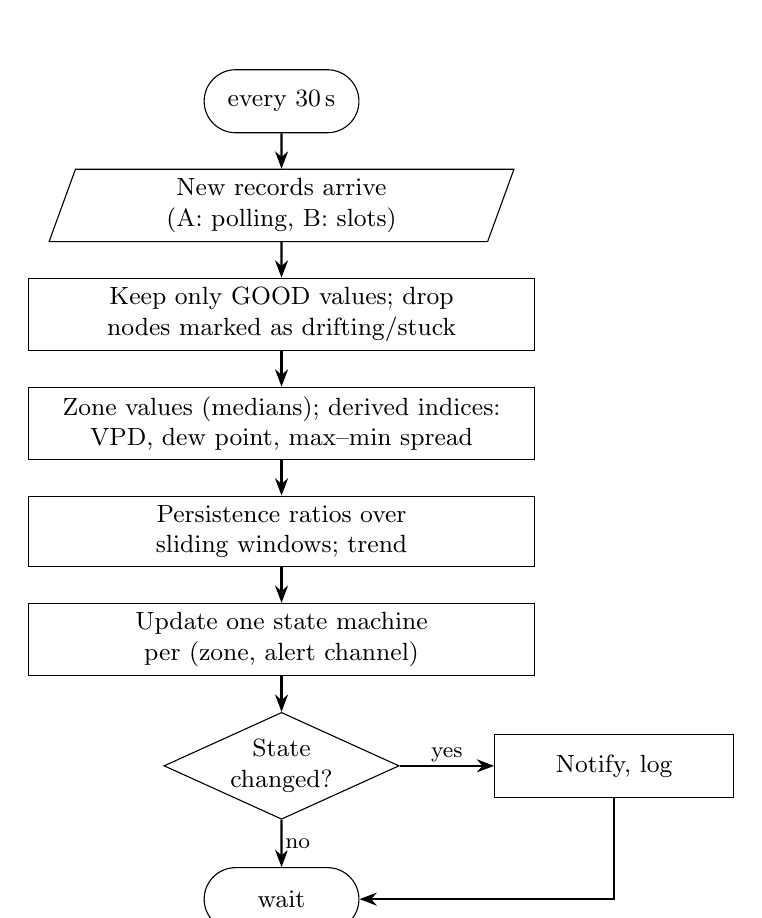
\begin{tikzpicture}[node distance=0.45cm]
  \node[term] (s) {every 30\,s};
  \node[io, below=of s, text width=5cm] (r) {New records arrive (A: polling, B: slots)};
  \node[proc, below=of r, text width=6.2cm] (q) {Keep only GOOD values; drop nodes marked as drifting/stuck};
  \node[proc, below=of q, text width=6.2cm] (c) {Zone values (medians); derived indices: VPD, dew point, max--min spread};
  \node[proc, below=of c, text width=6.2cm] (u) {Persistence ratios over sliding windows; trend};
  \node[proc, below=of u, text width=6.2cm] (f) {Update one state machine per (zone, alert channel)};
  \node[dec, below=of f] (d) {State\\changed?};
  \node[proc, right=1.2cm of d, text width=2.8cm] (n) {Notify, log};
  \node[term, below=0.6cm of d] (e) {wait};
  \draw[arr] (s) -- (r); \draw[arr] (r) -- (q); \draw[arr] (q) -- (c);
  \draw[arr] (c) -- (u); \draw[arr] (u) -- (f); \draw[arr] (f) -- (d);
  \draw[arr] (d) -- node[lbl, above]{yes} (n);
  \draw[arr] (d) -- node[lbl, right]{no} (e);
  \draw[arr] (n) |- (e);
\end{tikzpicture}
\caption{Alert analysis pipeline on the gateway}\label{fig:pipeline}
\end{figure}

\section{The alert state machine}
Each pair (zone, alert channel) -- for example ``zone Z2, high temperature'' -- has its own finite state machine (FSM). All FSMs follow the same template (Figure~\ref{fig:fsm}); only thresholds change. Three design choices:
\begin{itemize}
  \item \textbf{Moore outputs plus entry actions:} the lights and the siren are Moore outputs -- they depend only on the current state, so they do not flicker when data is noisy. Messages are \emph{entry actions}: sent once when a state is entered, plus a periodic reminder while in ALARM.UNACK.
  \item \textbf{Hierarchical:} NORMAL, WARNING and ALARM sit inside a MONITORING super-state. The transition to SENSOR\_FAULT is defined once, at the super-state level. ALARM has two sub-states: UNACK (siren on) and ACK (operator acknowledged; siren off, red light stays).
  \item \textbf{Clean inputs only:} the FSM sees zone values built from GOOD data, never a raw node reading.
\end{itemize}

\begin{figure}[htbp]
\centering
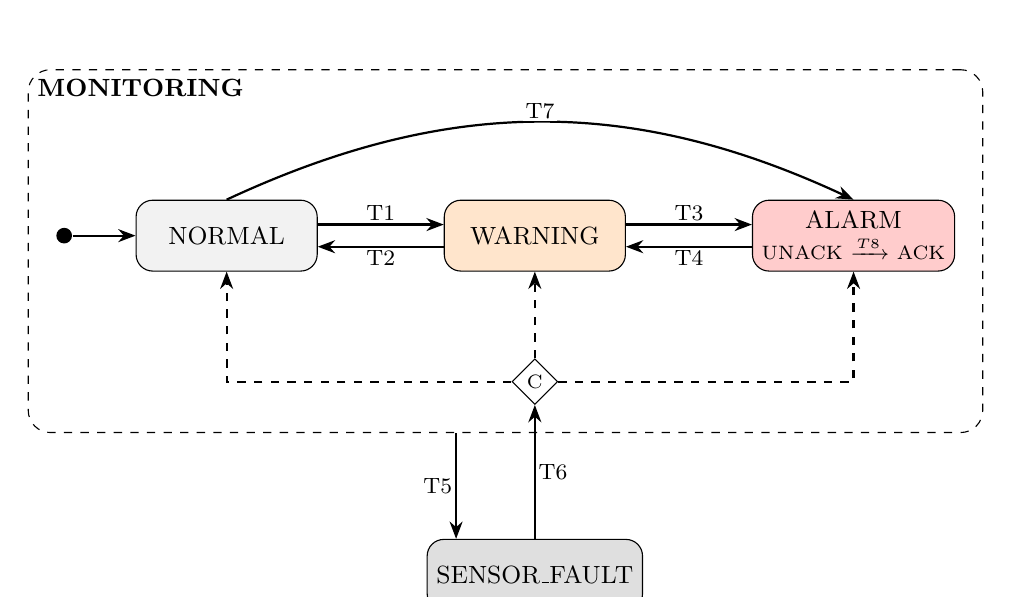
\begin{tikzpicture}[node distance=1.2cm and 1.6cm]
  \node[st, fill=gray!10] (nor) {NORMAL};
  \node[st, fill=orange!20, right=of nor] (war) {WARNING};
  \node[st, fill=red!20, right=of war] (ala) {ALARM\\{\scriptsize UNACK $\xrightarrow{T8}$ ACK}};
  \draw[arr] ([yshift=4pt]nor.east) -- node[lbl, above]{T1} ([yshift=4pt]war.west);
  \draw[arr] ([yshift=-4pt]war.west) -- node[lbl, below]{T2} ([yshift=-4pt]nor.east);
  \draw[arr] ([yshift=4pt]war.east) -- node[lbl, above]{T3} ([yshift=4pt]ala.west);
  \draw[arr] ([yshift=-4pt]ala.west) -- node[lbl, below]{T4} ([yshift=-4pt]war.east);
  \draw[arr] (nor.north) to[bend left=25] node[lbl, above]{T7} (ala.north);
  \node[draw, diamond, inner sep=1.5pt, font=\scriptsize, below=1.1cm of war] (c) {C};
  \draw[arr, dashed] (c.west) -| (nor.south);
  \draw[arr, dashed] (c) -- (war);
  \draw[arr, dashed] (c.east) -| (ala.south);
  \node[fill=black, circle, inner sep=2pt, left=0.8cm of nor] (ini) {};
  \draw[arr] (ini) -- (nor);
  \coordinate (top) at ($(war.north)+(0,1.3)$);
  \begin{scope}[on background layer]
    \node[draw, rounded corners=8pt, dashed, fit=(ini)(nor)(war)(ala)(c)(top), inner sep=0.35cm, label={[font=\small\bfseries, anchor=north west]north west:MONITORING}] (mon) {};
  \end{scope}
  \node[st, fill=gray!25, below=1.7cm of c] (flt) {SENSOR\_FAULT};
  \coordinate (f5) at ($(flt.north)+(-1.0,0)$);
  \draw[arr] (f5 |- mon.south) -- node[lbl, left]{T5} (f5);
  \draw[arr] (flt.north) -- node[lbl, right]{T6} (c.south);
\end{tikzpicture}
\caption{Hierarchical alert FSM (one zone, high-temperature channel); C is the choice point used when recovering from a sensor fault}\label{fig:fsm}
\end{figure}

\begin{table}[htbp]
\centering
\caption{Transitions of the high-temperature FSM}\label{tab:trans}
\small
\begin{tabularx}{\textwidth}{c >{\raggedright\arraybackslash}p{4.3cm} Y}
\toprule
\textbf{ID} & \textbf{Transition} & \textbf{Condition (``sustained'' is defined in Section~\ref{sec:persist})}\\
\midrule
T1 & NORMAL $\to$ WARNING & $T > 32$\,°C sustained over 5\,min\\
T2 & WARNING $\to$ NORMAL & $T < 30$\,°C sustained over 5\,min\\
T3 & WARNING $\to$ ALARM & $T > 35$\,°C sustained over 3\,min, \emph{or} rising trend (Section~\ref{sec:trend})\\
T4 & ALARM $\to$ WARNING & $T < 33$\,°C sustained over 5\,min\\
T7 & NORMAL $\to$ ALARM & $T > 35$\,°C sustained over 3\,min (sudden jump, no need to pass WARNING)\\
T8 & ALARM.UNACK $\to$ ALARM.ACK & Operator acknowledges\\
T5 & MONITORING $\to$ SENSOR\_FAULT & Zone INVALID, or DEGRADED with its two nodes disagreeing (Table~\ref{tab:zonevalid}), or too few recent samples\\
T6 & SENSOR\_FAULT $\to$ C & Reliable data is back; C re-enters ALARM, WARNING or NORMAL according to current data. A return to ALARM always enters \textbf{ALARM.UNACK} (siren on): an acknowledgement given before the fault may no longer apply\\
\bottomrule
\end{tabularx}
\end{table}

\why{The 32\,°C / 35\,°C levels are typical reference values for common vegetables and are \emph{configurable per crop}; the method does not depend on them. The exit levels (30\,°C, 33\,°C) are 2\,°C below the entry levels -- see hysteresis below.}

\textbf{Execution rules.}
\begin{itemize}[noitemsep]
  \item Each FSM moves at most one step per cycle. If several conditions hold, a fixed priority decides: sensor fault (T5) $>$ escalation (T7, T3) $>$ T1 $>$ de-escalation (T4, T2). The machine is therefore deterministic.
  \item \textbf{Escalate fast, de-escalate carefully:} there is a shortcut NORMAL $\to$ ALARM but no shortcut ALARM $\to$ NORMAL. Missing a danger is worse than clearing an alarm late.
  \item \textbf{Fail-safe:} missing data never leads to NORMAL; it leads to SENSOR\_FAULT, which is reported clearly.
  \item \textbf{Messages as entry actions}, with a reminder every 15 minutes while an alarm is unacknowledged -- no message flood.
\end{itemize}

\section{Four mechanisms against false alarms}\label{sec:persist}
\subsection{Persistence over a sliding window}
A condition (e.g.\ ``$T > 32$\,°C'') counts as \textbf{sustained} when
\begin{equation}
  \frac{\#\ \text{recent samples satisfying the condition}}{\#\ \text{recent samples available}} \;\geq\; 0.8,
\end{equation}
with at least 60\,\% of the expected samples available.
The window is 5\,min (10 samples) for WARNING and 3\,min (6 samples) for ALARM.

\why{\emph{80\,\% rather than 100\,\%:} one noisy or missing sample does not reset the count, so a real event is not delayed by a single glitch. \emph{At least 60\,\% available:} a decision made on too few samples is not trustworthy; below that, the zone goes to SENSOR\_FAULT instead. \emph{5 and 3 minutes:} misting or an opened door disturbs the air for a minute or two, while crop damage from heat needs longer exposure -- so a few minutes of confirmation removes most false alarms at little cost. ALARM uses the shorter window because it is the more dangerous level.}

\subsection{Hysteresis -- avoiding a ``Zeno'' alarm}
With a single threshold, a noisy value hovering around 32\,°C would switch the alarm on and off over and over -- in the ideal continuous model, infinitely often in finite time (a Zeno-like effect). Two things prevent this. First, the exit threshold is 2\,°C below the entry threshold, far larger than the noise of a zone value, so every change of state needs a real temperature swing of more than 2\,°C. Second, every transition needs a minimum amount of evidence, which bounds how fast states can change:
\begin{itemize}[noitemsep]
  \item de-escalation needs 8 of 10 samples beyond the exit level: at least 4\,min;
  \item escalation by threshold needs 5 of 6 samples above the ALARM level: at least 2.5\,min; escalation by trend needs the trend to hold for 3 cycles: at least 1.5\,min.
\end{itemize}
The fastest possible oscillation is WARNING $\to$ ALARM $\to$ WARNING, which takes at least $1.5 + 4 = 5.5$\,min for two changes, i.e.\ \textbf{at most about 22 changes per hour per channel} (about 18 if the trend rule is not involved). This is a finite bound, so there is no Zeno behaviour; in the simulation the real number was far lower (Chapter~\ref{ch:pe}).

\subsection{Zone median}
As shown in Section~\ref{sec:zone}, while a zone is VALID ($\geq 3$ GOOD nodes) one wrong node cannot move the zone value, so a single faulty sensor cannot raise an alarm. With only 2 GOOD nodes the zone value is used only if they agree within 1\,°C.

\subsection{Late data is not missing data (watermark)}
The persistence ratio uses \emph{the most recent samples that have actually arrived}, looking back over the window plus the design's expected delivery delay (the \emph{watermark}): one cycle for A, one report period plus slot waiting for B. Early data (always in A; in B's dense mode) is used immediately, so alerts are not slowed down. Data that is simply not due yet (PENDING) is not counted as missing, so B does not fall into false sensor faults.

\why{Without this rule, a version of the simulation of Design B (120\,s report period) with a plain clock-aligned window produced about five times as many state changes as Design A -- roughly 180 instead of 36 per week, mostly false SENSOR\_FAULT entries -- the gateway kept mistaking ``not sent yet'' for ``lost''. This is a concrete example of the communication design and the analysis design interacting, found only by evaluation (Chapter~\ref{ch:pe}).}

\section{Keeping real alarms fast}\label{sec:trend}
\begin{itemize}
  \item \textbf{Trend alert.} If the zone temperature has risen by more than 2\,°C in 10 minutes -- computed as the median of the last 3 minutes minus the median of 3 minutes taken 10 minutes earlier, and holding for 3 consecutive cycles -- WARNING escalates to ALARM \emph{before} 35\,°C is reached. Medians and the 3-cycle requirement stop a short misting dip from faking a trend.
  \item \textbf{Shortcut} NORMAL $\to$ ALARM for sudden jumps.
  \item \textbf{Shorter window} for ALARM than for WARNING.
  \item \textbf{The gateway watches itself:} a hardware watchdog relay sounds the siren if the gateway software stops, and a heartbeat to the outside reports a dead gateway.
\end{itemize}

\why{\emph{2\,°C in 10 minutes:} the normal morning warm-up is a fraction of a degree per 10 minutes, whereas a failed fan heats the air several times faster. 2\,°C separates the two clearly.}

\section{Alerts from derived indices and from space}\label{sec:derived}
Raw thresholds miss some risks, so the gateway also computes:
\begin{itemize}
  \item \textbf{Vapour pressure deficit (VPD)} -- how strongly the air ``pulls'' water from leaves:
  \begin{equation}
    e_s = 0.6108\,\exp\!\left(\frac{17.27\,T}{T + 237.3}\right)\ \text{kPa}, \qquad VPD = e_s\left(1 - \frac{RH}{100}\right).
  \end{equation}
  Too low: fungal disease risk; too high: plant water stress. Neither is visible from temperature or humidity alone.
  \item \textbf{Dew-point margin} $T - T_d$ (Magnus formula): when it is small, water condenses on leaves, typically at night.
  \item \textbf{Daily light integral (DLI):} plants need a total amount of photosynthetic light per day, not a momentary value. The TSL2591 measures lux, so we convert with the usual factor for \emph{sunlight}, $\mathrm{PPFD} \approx E_{lux}/54$\,µmol\,m\textsuperscript{-2}\,s\textsuperscript{-1} (1\,klux $\approx$ 18.5\,µmol\,m\textsuperscript{-2}\,s\textsuperscript{-1}), and sum over the day:
  \begin{equation}
    DLI = \sum_k \mathrm{PPFD}_k \cdot \Delta t_k \cdot 10^{-6}\ \ \text{mol\,m}^{-2}\,\text{day}^{-1},
  \end{equation}
  checked once in the evening. The factor depends on the light spectrum: it is only approximate under shading nets and wrong for LED grow lights, where a lamp-specific factor or a PAR (quantum) sensor is needed.
  \item \textbf{Uneven temperature:} the spread between the hottest and coldest GOOD nodes. A large spread usually means a fan or vent in one area has failed -- an alert that only a multi-point system can give.
\end{itemize}
All use the same FSM template (WARNING level only), with windows adapted to how slowly each quantity changes.

\section{Device and Infrastructure Diagnostics}\label{sec:devdiag}
Environmental alerts (``the greenhouse is too hot'') and device health alerts (``a sensor is broken'') are segregated into distinct channels, ensuring that agricultural operators are not inundated with technical telemetries while maintenance technicians receive actionable diagnostic data:
\begin{itemize}[noitemsep]
  \item \textbf{Both designs:} drifting or stuck sensor; zone in SENSOR\_FAULT; gateway watchdog heartbeat loss.
  \item \textbf{Design A only:} cable continuity break with exact segment localization; rising CRC error rate (indicating moisture ingress in a cable gland).
  \item \textbf{Design B only:} low battery voltage ($V_{\text{bat}} < 3.10\,\text{V}$); declining link margin (canopy wetting); packet integrity fault; node slot desynchronization.
\end{itemize}

\section{Operations and Maintenance (O\&M): Notification Hierarchy, Dashboard, and SOPs}\label{sec:om}
A resilient embedded system must define clear post-deployment operational workflows. Rather than relying on generic ``text messages'', our architecture incorporates a role-based notification hierarchy, a four-tier dispatch system, dedicated visual dashboards, and formal Standard Operating Procedures (SOPs).

\subsection{Stakeholder Hierarchy and Multi-Channel Notification Matrix}
Field operations involve three distinct stakeholder roles:
\begin{enumerate}[noitemsep]
  \item \textbf{On-site Worker / Night Guard (Worker):} Present on farm grounds; responsible for immediate physical interventions (manual curtain roll-up, emergency misting, fan circuit breaker check).
  \item \textbf{Farm Owner / Head Agronomist (Agronomist):} Manages crop climate recipes and economic yields; reviews daily growth trends (VPD, DLI); acts as primary escalation contact.
  \item \textbf{Systems Maintenance Technician (Technician):} Responsible for hardware uptime, sensor cleaning, battery swapping, cable repairs, and gateway servicing.
\end{enumerate}

\begin{table}[htbp]
\centering
\caption{Role-based notification matrix and automated escalation policy}\label{tab:notify}
\small
\begin{tabularx}{\textwidth}{>{\raggedright\arraybackslash}p{2.6cm} >{\raggedright\arraybackslash}p{1.8cm} >{\raggedright\arraybackslash}p{3.0cm} >{\raggedright\arraybackslash}p{3.4cm} Y}
\toprule
\textbf{Event Severity} & \textbf{Target Role} & \textbf{Dispatch Channel} & \textbf{Field Action Required} & \textbf{Escalation Policy}\\
\midrule
\textbf{CRITICAL ALARM}\newline ($T > 35^\circ\text{C}$, severe freeze $< 2^\circ\text{C}$) & Worker \newline+ Agronomist & Local Strobe/Siren (85\,dB) \newline+ Cellular SMS / Auto-Call \newline+ Telegram push & Immediate physical inspection of cooling pads, fans, and vents; acknowledge on gateway & If unacknowledged within 5\,min, automated voice dialer calls Agronomist; repeats every 3\,min\\
\midrule
\textbf{WARNING / TREND}\newline ($T > 32^\circ\text{C}$, VPD stress, DLI deficit) & Agronomist & Web Dashboard \newline+ Daily Telegram/Zalo digest & Review climate trajectory; adjust shading net or misting schedule & Logged to dashboard; no audible siren; digest at 18:00 daily\\
\midrule
\textbf{SENSOR FAULT}\newline (Stuck reading, drift $> 2^\circ\text{C}$, offline) & Technician & Telegram Bot maintenance channel + Gateway UI & Clean SHT40 filter; inspect cable gland; execute recalibration & Auto-quarantines node; repeats notification at 08:00 daily until resolved\\
\midrule
\textbf{LOW BATTERY (B)}\newline ($V_{\text{bat}} < 3.10\,\text{V}$,\newline $\text{SOC} < 15\,\%$) & Technician & Maintenance dashboard \newline+ Telegram bot message & Hot-swap 18650 cell within 48\,h; inspect solar panel surface & Node enters low-power sleep (reports every 15\,min); reminds at 24\,h\\
\midrule
\textbf{CABLE BREAK (A)}\newline (P2 continuity lost) & Technician & SMS + Maintenance panel & Inspect identified inter-node cable segment; re-splice cable & Ring bus automatically splits into dual stubs (zero data loss); alert remains active\\
\midrule
\textbf{GATEWAY DOWN}\newline (Heartbeat lost) & Agronomist \newline+ Technician & Cellular SMS from external cloud heartbeat monitor & Inspect AC mains power; check UPS battery; restart gateway & Standalone hardware relay sounds backup horn after 3\,min silence\\
\bottomrule
\end{tabularx}
\end{table}

\subsection{Multi-Tier Notification Dispatch Architecture}
The gateway implements four complementary notification tiers to ensure delivery under severe physical conditions:
\begin{itemize}
  \item \textbf{Tier 1: Local Physical Annunciator (Gateway Exterior):} An industrial 24\,V LED flashing strobe and an 85\,dB piezo buzzer mounted outside the greenhouse door. Driven directly by a fail-safe hardware relay on the gateway, this tier operates with \emph{zero network dependencies}, alerting on-site workers instantly even during complete internet, cellular, and electrical grid outages.
  \item \textbf{Tier 2: Direct Cellular GSM/4G SMS and Auto-Dialer:} An onboard Quectel EC25 LTE module with fallback to 2G/3G communicates directly via AT commands. Critical alarms bypass the local internet router, transmitting high-priority SMS alerts and initiating automated voice phone calls directly to the grower's mobile phone within 15 seconds.
  \item \textbf{Tier 3: Over-the-Top Messaging (Telegram Bot / Zalo Webhook):} For informational warnings, daily climate digests, and hardware maintenance tickets, the gateway posts structured rich-text messages with graphical thumbnails and inline interactive buttons (e.g., \textsf{[Acknowledge Alarm]}, \textsf{[Mute Siren 15 min]}, \textsf{[View Zone Z2 Graph]}).
  \item \textbf{Tier 4: Local and Cloud Web Dashboard (Grafana):} A lightweight web server (NGINX + Grafana) hosted locally on the gateway's embedded Linux board. Operators access real-time spatial heatmaps, zone time-series curves, battery state-of-charge gauges, and FSM alert states from any smartphone or tablet connected to the local greenhouse Wi-Fi, with background synchronization to an off-site cloud server when WAN is available.
\end{itemize}

\subsection{Standard Operating Procedures (SOPs) for Field Maintenance}
To prevent alert fatigue and ensure prompt remediation, three standard operational procedures are codified:

\subsubsection{SOP-01: Low-Battery Replacement and Solar Servicing (Design B)}
\begin{enumerate}[noitemsep]
  \item \textbf{Automated preservation:} When cell voltage drops below $3.10\,\text{V}$ (or after two consecutive days where peak voltage fails to exceed $3.25\,\text{V}$ due to cell aging or severe solar panel soiling), node firmware enters \emph{battery preservation mode}: it shuts down the light sensor, disables radio listen slots, and reports only a single diagnostic frame every 15 minutes.
  \item \textbf{Dispatch:} The Telegram bot sends a maintenance ticket specifying the node identifier and coordinates: \textsf{"[BATTERY WARNING] Node N07 (Zone Z2, East Column, y = 20.8 m) cell voltage = 3.08 V. Replace cell within 48 hours."}
  \item \textbf{Field execution:} The technician carries a pre-charged 18650 LiFePO$_4$ cell from the gateway charging dock. Without dismounting the enclosure, the technician releases the four IP65 stainless steel quick-latches, extracts the depleted cell from its reverse-polarity protected holder, and inserts the fresh cell ($< 90$\,seconds downtime).
  \item \textbf{Solar panel hygiene:} The technician wipes dust, chemical spray residue, and algae off the 1.5\,W panel cover with a damp microfiber cloth.
  \item \textbf{Verification:} Upon battery insertion, the node executes a 3-second self-test LED sequence, transmits an immediate commissioning frame to the gateway, and resumes standard 30\,s adaptive operation. The gateway automatically clears the ticket and logs the replacement.
\end{enumerate}

\subsubsection{SOP-02: Sensor Fault Resolution and Recalibration}
\begin{enumerate}[noitemsep]
  \item \textbf{Isolation:} If a sensor reading deviates by $> 2.0^\circ\text{C}$ from its zone median for 10 minutes or remains statically frozen for 30 minutes, the gateway flags the node as \texttt{SUSPECT} and removes its weight from the zone median voting ($M-1$ fallback).
  \item \textbf{Condensation recovery:} The technician issues a remote command via the dashboard to activate the SHT40's internal $200\,\text{mW}$ resistive heating element for 5 seconds to evaporate water droplets trapped inside the sintered PTFE filter membrane.
  \item \textbf{Probe replacement:} If the sensor remains degraded after heating, the technician inspects the probe. The SHT40/TSL2591 assembly is connected via a waterproof M12 quick-disconnect connector, allowing the entire sensor head to be hot-swapped in 2 minutes without opening the main MCU enclosure or re-flashing firmware.
\end{enumerate}

\subsubsection{SOP-03: Cable Break Localization and Splicing (Design A)}
\begin{enumerate}[noitemsep]
  \item \textbf{Automated ring split:} When gateway Port P2 ceases receiving Modbus carrier from Port P1, the gateway continuity monitor trips, immediately engaging Split Mode (polling odd nodes via P1 and even nodes via P2).
  \item \textbf{Localization ticket:} The gateway identifies the break between the last responding node on P1 and the last responding node on P2 (e.g., \textsf{"[CABLE BREAK] Bus severed between Node N06 (East, y=20.8 m) and Node N04 (East, y=29.2 m). All nodes remain operational."})
  \item \textbf{Physical repair:} The technician walks the 8.3\,m PVC conduit run between N06 and N04, checks for tilling blade damage or loose junction boxes, splices the 2-pair STP cable with an IP68 gel-filled inline closure, and re-attaches the shield drain wire. Normal ring continuity is restored automatically.
\end{enumerate}

\subsection{Audit Logging and Data Retention Policy}
The gateway maintains an embedded time-series database (SQLite / DuckDB) storing three retention tiers:
\begin{itemize}[noitemsep]
  \item \textbf{High-resolution buffer (30\,s data):} Retained locally for 90 days ($\approx 450\,\text{MB}$ total storage); used for short-term agronomic correlation and fault investigation.
  \item \textbf{Daily climate aggregates:} Daily minimum, maximum, mean, DLI, and VPD values are retained indefinitely ($< 10\,\text{MB}$ per year).
  \item \textbf{Immutable event log:} Every FSM state transition, siren activation, operator acknowledgment (logging whether ACK was initiated via the physical gateway push-button or a mobile app token), and sensor fault ticket is recorded in a tamper-evident event table for post-incident insurance and operational review.
\end{itemize}

% ============================================================
\chapter{Performance Evaluation}\label{ch:pe}
% ============================================================
The three mechanisms above were evaluated with the standard 10-step performance-evaluation procedure. Table~\ref{tab:pe} summarises the steps; the metrics are chosen \emph{separately} for each design because each design can fail in different ways.

\section{The 10 steps in brief}
\begin{table}[htbp]
\centering
\caption{The 10-step evaluation applied to A and B}\label{tab:pe}
\small
\begin{tabularx}{\textwidth}{>{\raggedright\arraybackslash}p{2.7cm} Y}
\toprule
\textbf{Step} & \textbf{Our choice}\\
\midrule
1. Goals, system & Compare A and B fairly (stated neutrally, not ``prove B is better''); tune each design's parameters. System = nodes + network + gateway. The phone network and the Internet are outside: their delay does not depend on A or B.\\
2. Services, outcomes & Data collection, alerting, fault diagnosis. Each can succeed, go wrong (wrong/late value, false alarm), or fail (lost data, missed alarm).\\
3. Metrics & One metric per outcome (Table~\ref{tab:metrics}); separate sets for A and B.\\
4. Parameters & System: window lengths, thresholds, bus speed (A), report period and radio settings (B). Workload: daily temperature cycle, fan failures, misting, sensor noise and faults, packet loss.\\
5. Factors & Design (A/B); trend alert on/off; B: report period, dense mode on/off, packet-loss rate; node density ($N \in \{6, 8, 10, 12, 16, 20\}$); plus a naive single-threshold baseline.\\
6. Technique & Analytical models first (bus timing, link budget, collisions, energy), then simulation for time-dependent behaviour, then measurement on a prototype (planned). Each technique cross-checks another.\\
7. Workload & 7 simulated days: daily cycle close to the warning level, 2 fan failures per week, misting 3 times a day, sensor spikes, one drifting and one stuck sensor, random packet loss.\\
8. Experiments & 12 main configurations $\times$ 10 repetitions, plus 6 sensitivity runs for node density ($N=6\dots 20$). Repetition $r$ uses common random numbers to isolate design effects.\\
9. Analysis & Mean with 95\,\% confidence interval, plus the worst case (for alarms, the worst case matters most).\\
10. Presentation & Tables and a chart (below).\\
\bottomrule
\end{tabularx}
\end{table}

\section{Metrics chosen for each design}
\begin{table}[htbp]
\centering
\caption{Metrics per design and why}\label{tab:metrics}
\small
\begin{tabularx}{\textwidth}{>{\raggedright\arraybackslash}p{2.2cm} Y Y}
\toprule
& \textbf{Metrics} & \textbf{Why this set}\\
\midrule
Both designs & Alert delay (mean and worst); false alarms; missed events; number of state changes; measurement error; fault-detection time; data completeness & These are the outcomes of the three services; they are used to compare A with B\\
Design A only & Poll cycle time and bus load; nodes still reachable after a cable break; voltage at the last node & A's weak point is correlated failure (a cable break), not energy. Data age is excluded: it is constant in A\\
Design B only & Link-layer delivery ratio; collision probability; transmissions per node per day; average current / autonomy; link margin; fairness of delivery across nodes (Jain index) & B's weak points are the shared radio channel and the battery. Link margin is ``nominal-is-best'': too low loses packets, too high wastes energy. The fairness index reveals a single far node that keeps losing packets, which an average would hide\\
\bottomrule
\end{tabularx}
\end{table}

\section{Key results}
The results below come from our discrete-event simulation model (\texttt{greenhouse\_sim.py}). ``$x \pm y$'' means mean $\pm$ half-width of the 95\,\% confidence interval over the repetitions.

\begin{table}[htbp]
\centering
\caption{Key simulation results}\label{tab:results}
\small
\begin{tabularx}{\textwidth}{>{\raggedright\arraybackslash}p{4.3cm} >{\raggedright\arraybackslash}p{4.4cm} Y}
\toprule
\textbf{Question} & \textbf{Result} & \textbf{Meaning}\\
\midrule
Does node filtering work? (criterion 2) & Error of one reading 0.67\,°C $\to$ after median 0.08\,°C & Occasional spikes dominate the raw error; the median removes them\\
Are faulty sensors caught? (criterion 2) & Stuck: after 30\,min. Drift: caught at about 2.3\,°C offset & Matches the 30\,min / 2\,°C rules; caught before the error becomes harmful\\
Does the alert logic prevent flip-flopping? (criterion 3) & State changes per week, 3 zones: naive threshold $576 \pm 79$, our design $35 \pm 6$ & The remaining changes are genuine warm afternoons crossing 32\,°C\\
Are real events caught? (criterion 3) & 20 of 20 fan failures detected, 0 false ALARMs, in every configuration & The false-alarm filters do not hide real events\\
\bottomrule
\end{tabularx}
\end{table}

\subsection{Does the network change the alert delay? (paired comparison)}
Because every configuration was run on the \emph{same} 20 fan failures (common random numbers), the fair way to compare two designs is per event: compute ``delay of B $-$ delay of A'' for each of the 20 failures, then a confidence interval on that difference. This removes the event-to-event variation that both designs share, and is much more precise than comparing two separate intervals.

\begin{table}[htbp]
\centering
\caption{Alert delay and paired differences (20 fan failures; trend alert off unless stated)}\label{tab:paired}
\small
\begin{tabularx}{\textwidth}{>{\raggedright\arraybackslash}p{3.9cm} c c >{\raggedright\arraybackslash}p{3.2cm} Y}
\toprule
\textbf{Configuration} & \textbf{Mean delay} & \textbf{Worst} & \textbf{Paired vs.\ A (95\,\% CI)} & \textbf{Reading}\\
\midrule
A (RS-485) & $2.70 \pm 0.37$ & 6.0 & -- & Reference\\
B, fixed 30\,s & $2.75 \pm 0.43$ & 6.5 & $+0.05\ [-0.02, +0.12]$ & No significant difference\\
B, adaptive (120\,s + dense) & $2.75 \pm 0.43$ & 6.5 & $+0.05\ [-0.02, +0.12]$ & No significant difference; at most $\approx$7\,s slower\\
B, fixed 120\,s & $3.40 \pm 0.53$ & 7.5 & $+0.70\ [+0.43, +0.97]$ & Significantly slower; worst case near the 8\,min limit\\
\midrule
A, trend on & $-1.23 \pm 0.74$ & 1.5 & -- & Alarm before 35\,°C is reached\\
B adaptive, trend on & $-0.38 \pm 0.80$ & 3.0 & $+0.85\ [+0.61, +1.09]$ & Significantly later than A, but still before 35\,°C on average\\
\bottomrule
\end{tabularx}
\end{table}

\why{\emph{Alert delay} (minutes) is measured from the moment the true zone temperature crosses 35\,°C to the moment the FSM enters ALARM; it excludes SMS delivery. About 2.5\,min of it is intentional: the 3-minute ALARM window must see 5 of 6 samples above 35\,°C. So A's 2.7\,min is almost entirely the design's own confirmation time, not network delay -- which is why B can match it. A \emph{negative} delay means the trend rule raised the alarm before 35\,°C was reached. The trend rule looks 10 minutes back, and B's older samples are still sparse at that point, so B's trend alarm comes about 50\,s later than A's.}

\subsection{Does adaptive reporting save energy? (criterion 1)}
The fair baseline for adaptive reporting is the fixed schedule that gives the \emph{same alert delay}: sending every sample, every 30\,s. Table~\ref{tab:paired} shows that their delays are identical for every one of the 20 failures (paired difference exactly 0).

\begin{table}[htbp]
\centering
\caption{Transmissions per node per day (5\,\% packet loss, retries included)}\label{tab:tx}
\small
\begin{tabular}{l c c}
\toprule
\textbf{Reporting policy} & \textbf{Transmissions/node/day} & \textbf{Mean delay (trend off)}\\
\midrule
Fixed 30\,s (same-delay baseline) & 3{,}031 & 2.75\,min\\
\textbf{Adaptive: 120\,s + dense near thresholds} & \textbf{1{,}280 ($-58$\,\%)} & \textbf{2.75\,min}\\
Fixed 120\,s & 758 & 3.40\,min\\
\bottomrule
\end{tabular}
\end{table}

\why{\emph{3{,}031:} one sample every 30\,s is 2{,}880 packets a day, plus about 5\,\% retransmissions. \emph{1{,}280:} sparse packets every 120\,s (720 a day) plus dense packets during the warm hours when values are within 1\,°C of the warning level. Since the radio dominates the node's energy, 58\,\% fewer packets means roughly half the radio energy for the same alert delay. Fixed 120\,s is cheaper still, but significantly slower (Table~\ref{tab:paired}).}

\begin{figure}[htbp]
\centering
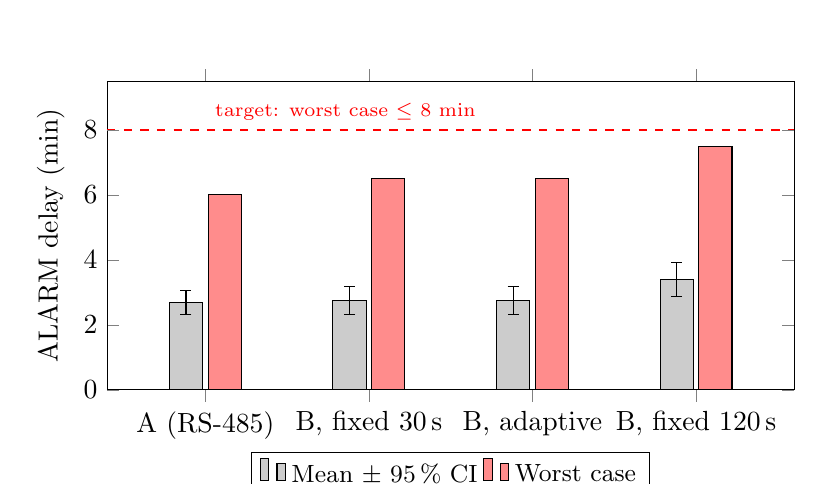
\begin{tikzpicture}
\begin{axis}[
  ybar, width=0.85\textwidth, height=5.5cm, bar width=12pt,
  ylabel={ALARM delay (min)}, ymin=0, ymax=9.5,
  symbolic x coords={A, B30, Bad, B120},
  xticklabels={A (RS-485), {B, fixed 30\,s}, {B, adaptive}, {B, fixed 120\,s}},
  xtick=data, enlarge x limits=0.2,
  legend style={at={(0.5,-0.2)}, anchor=north, legend columns=2, font=\small},
  error bars/y dir=both, error bars/y explicit,
  extra y ticks={8}, extra y tick labels={}, extra y tick style={grid=major, grid style={red, dashed}}
]
\addplot[fill=gray!40] coordinates {(A,2.70) +- (0,0.37) (B30,2.75) +- (0,0.43) (Bad,2.75) +- (0,0.43) (B120,3.40) +- (0,0.53)};
\addplot[fill=red!45] coordinates {(A,6.0) (B30,6.5) (Bad,6.5) (B120,7.5)};
\legend{Mean $\pm$ 95\,\% CI, Worst case}
\node[font=\scriptsize, red, anchor=south west] at (axis cs:A,8) {target: worst case $\leq$ 8 min};
\end{axis}
\end{tikzpicture}
\caption{Alert delay with the trend alert switched off (isolates the effect of the network)}\label{fig:delay}
\end{figure}

\subsection{Sensitivity analysis: node density and zone granularity (N = 6 to 20)}\label{sec:nodesens}
In Section~\ref{sec:arch}, we selected a $2\times6$ grid (12 nodes) by dividing the greenhouse into three zones of 4 nodes each. To verify whether 12 nodes is the right choice, we ran a sensitivity test across six grid configurations ($N \in \{6, 8, 10, 12, 16, 20\}$) in our simulation environment over the $20\times50$\,m area ($1{,}000\,\text{m}^2$). 

We evaluated each density on four practical criteria:
\begin{enumerate}[noitemsep]
  \item \textbf{Spatial interpolation error (RMSE):} Root Mean Square Error ($^\circ\text{C}$) over the greenhouse against the simulated solar and ventilation gradient ($28$--$32^\circ\text{C}$).
  \item \textbf{Hotspot detection delay ($t_{\text{detect}}$):} Time in minutes until a node detects a fan failure near the north wall ($(x, y) = (17, 45)$), which generates a local hot plume ($\Delta T = 6^\circ\text{C}$, radius $6$\,m, heating rate $0.8^\circ\text{C}$/min).
  \item \textbf{Zone voting availability ($P_{\text{valid}}$):} Probability that every zone retains at least 3 working nodes for majority voting under a 5\,\% random sensor failure rate ($P = [B(M, \geq 3)]^{\text{Zones}}$).
  \item \textbf{Network load and cost:} Initial equipment cost (Design B) and TDMA channel occupancy in the 30\,s frame.
\end{enumerate}

\begin{table}[htbp]
\centering
\caption{Sensitivity analysis across node densities ($N = 6$ to $20$) in a $20\times50$\,m greenhouse}\label{tab:nodesens}
\small
\setlength{\tabcolsep}{3.5pt}
\begin{tabular}{c c c c c c c c c}
\toprule
\textbf{$N$} & \textbf{Grid} & \textbf{Zones ($M$)} & \textbf{$d_{\max}$ (m)} & \textbf{RMSE ($^\circ\text{C}$)} & \textbf{$t_{\text{detect}}$ (min)} & \textbf{$P_{\text{valid}}$ (\%)} & \textbf{CAPEX (USD)\textsuperscript{*}} & \textbf{TDMA Load\textsuperscript{*}}\\
\midrule
6  & $2\times3$  & 2 ($M=3$) & 9.72 & 0.639 & 5.79 & 73.5 & \$315.10 & 35.0\,\%\\
8  & $2\times4$  & 2 ($M=4$) & 8.00 & 0.601 & 3.41 & 97.2 & \$373.70 & 45.0\,\%\\
10 & $2\times5$  & 2 ($M=5$) & 7.07 & 0.586 & 3.12 & 99.8 & \$432.30 & 55.0\,\%\\
\textbf{12} & \textbf{$2\times6$} & \textbf{3 ($M=4$)} & \textbf{6.51} & \textbf{0.578} & \textbf{3.24} & \textbf{95.9} & \textbf{\$490.90} & \textbf{65.0\,\%}\\
16 & $2\times8$  & 4 ($M=4$) & 5.90 & 0.571 & 3.80 & 94.5 & \$608.10 & 85.0\,\%\\
20 & $2\times10$ & 4 ($M=5$) & 5.59 & 0.569 & 4.42 & 99.5 & \$725.30 & 105.0\,\%\\
\bottomrule
\multicolumn{9}{p{0.96\textwidth}}{\footnotesize\textsuperscript{*}Includes $N$ indoor nodes plus 1 outdoor reference node (N00) and Gateway (\$110.00), harmonized with Table~\ref{tab:bom}. TDMA Load is $(N+1)/20$ slots in the 30\,s frame ($1.5\,\text{s}/\text{slot}$). At $N=20$, channel load reaches 105.0\,\% (21 slots), exceeding frame capacity.}\\
\end{tabular}
\end{table}

\textbf{Why 12 nodes ($2\times6$ grid) is the most balanced choice:}
\begin{itemize}
  \item \textbf{Diminishing returns in temperature accuracy:} Increasing from $N=6$ to $N=12$ reduces interpolation error from $0.64^\circ\text{C}$ to $0.58^\circ\text{C}$ and shortens the maximum distance to the nearest sensor from 9.7\,m to 6.5\,m. Adding more nodes beyond 12 ($N=16$) only reduces RMSE by another $0.007^\circ\text{C}$---which is negligible compared to the sensor's $\pm 0.1^\circ\text{C}$ accuracy---while increasing hardware cost by 23.9\,\% (\$117.20).
  \item \textbf{Zone size and fault tolerance:} Configurations with $N=8$ or $N=10$ nodes can only be divided into two $500\,\text{m}^2$ zones. A 25\,m long zone is too large: localized temperature variations get smoothed out by the median calculation. Twelve nodes is the minimum number that supports three separate zones ($333\,\text{m}^2$ each) with 4 nodes per zone, ensuring that majority voting still functions reliably if one sensor fails (95.9\,\% probability).
  \item \textbf{TDMA channel capacity:} In Design B's 30\,s frame (20 slots $\times$ 1.5\,s), $N=12$ (13 dedicated slots used, including the outdoor node N00) consumes 65.0\,\% of the frame. This leaves 5 spare slots for expansion and 2 shared slots for urgent alarms. With $N=16$, channel occupancy reaches 85.0\,\%, leaving little room for retries; and $N=20$ (21 slots) exceeds the 30\,s frame completely (105.0\,\% load).
\end{itemize}
In summary, 12 nodes provide adequate spatial accuracy, reliable 3-zone majority voting, and a comfortable 65\,\% TDMA channel margin, without unnecessary hardware expenditure.

\section{Evaluation changed the design}
The evaluation was not only a final check -- it fixed three design flaws, all caused by the interaction between communication and alert analysis:
\begin{enumerate}[noitemsep]
  \item B with sparse reporting and a clock-aligned window caused false SENSOR\_FAULT states (about 180 instead of 36 state changes per week) $\Rightarrow$ the watermark and the PENDING quality level were added.
  \item The first watermark version made B slower than A $\Rightarrow$ it was changed to use ``the most recent samples that have arrived''.
  \item Sending a single early packet when nearing a threshold did not reduce delay, because persistence needs several fresh samples $\Rightarrow$ replaced by dense mode.
\end{enumerate}
The simulation covers the high-temperature channel under both independent and burst loss models. Physical validation on a pilot prototype (one zone per design over two weeks, featuring a reference thermometer, power consumption logging, cable-cut and gateway-reboot drills) is scheduled prior to commercial deployment to empirically confirm these findings.

\section{Stress Testing Under Correlated Packet Loss}\label{sec:threats}
An important limitation of the simulation results in Table~\ref{tab:paired} is the assumption of independent 5\,\% random packet loss. Under independent random loss, the probability of collecting at least 5 out of 6 samples in the 3-minute alert window is about 96.7\,\%, which allows Design B to easily match Design A's delay.

In a real greenhouse, radio signal drops caused by water droplets and wet leaves do not occur independently. Instead, losses happen in continuous bursts:
\begin{itemize}[noitemsep]
  \item \textbf{Overhead misting passes:} Automated spray nozzles generate airborne water droplets that attenuate 923\,MHz signals by an estimated 15--20\,dB for 2--4 continuous minutes.
  \item \textbf{Morning dew condensation:} Thick water films on plant leaves create prolonged multipath fading until the morning sun evaporates surface moisture.
\end{itemize}

\emph{Methodological note:} As with the link budget's 25--35\,dB foliage attenuation, these burst fade scenarios and loss probabilities are assumed stress-testing parameters designed to explore system boundaries, not empirical on-site RF channel measurements. Their purpose is sensitivity analysis---determining at what outage duration wireless alert latency exceeds crop safety margins.

\subsection{Testing with Burst Loss (Gilbert-Elliott Model)}
To evaluate how Design B behaves during sustained fades, we simulated both designs using a standard two-state Gilbert-Elliott Markov channel model (1{,}000 heating spike trials):
\begin{itemize}[noitemsep]
  \item \textbf{Good state ($G$):} Clean channel, background packet loss $P(\text{loss}|G) = 2\,\%$.
  \item \textbf{Bad state ($B$):} Severe misting or condensation fade, loss $P(\text{loss}|B) = 90\,\%$, with average burst duration $T_{\text{burst}} \in \{0, 2, 5\}\,\text{min}$.
\end{itemize}

\begin{table}[htbp]
\centering
\caption{Stress testing ALARM delay under correlated foliage burst losses (1{,}000 heating spike trials)}\label{tab:stress}
\small
\begin{tabularx}{\textwidth}{l c c c Y}
\toprule
\textbf{Channel Condition} & \textbf{Design} & \textbf{Mean Delay} & \textbf{95th Percentile} & \textbf{Physical Interpretation / Agronomic Impact}\\
\midrule
\multirow{2}{*}{\makecell[l]{Nominal i.i.d.\\5\,\% loss}} & A (Wired) & $2.70 \pm 0.37$\,min & 6.0\,min & Hardware poll; constant latency\\
 & B (LoRa) & $2.65 \pm 0.15$\,min & 3.0\,min & Dense mode easily masks scattered packet drops\\
\midrule
\multirow{2}{*}{\makecell[l]{2-min Correlated\\Burst (Misting)}} & A (Wired) & $2.70 \pm 0.37$\,min & 6.0\,min & Completely immune to airborne water droplets\\
 & B (LoRa) & $4.36 \pm 0.32$\,min & 5.0\,min & Overhead misting cycle delays ALARM confirmation by $+1.66$\,min\\
\midrule
\multirow{2}{*}{\makecell[l]{5-min Correlated\\Burst (Dew Fade)}} & A (Wired) & $2.70 \pm 0.37$\,min & 6.0\,min & Unaffected; deterministic cycle preserved\\
 & B (LoRa) & $6.96 \pm 0.48$\,min & 7.5\,min & Prolonged condensation pushes delay dangerously close to 8\,min crop limit\\
\bottomrule
\end{tabularx}
\end{table}

\textbf{Key findings from burst-loss testing:}
\begin{enumerate}
  \item \textbf{Impact of burst duration on alarm timing:} Design B matches Design A only when packet losses are scattered or burst outages remain under 2 minutes. When overhead misting creates a 2-minute fade, Design B's average alert delay increases from 2.65\,min to 4.36\,min. Under a 5-minute fade, delay reaches 6.96\,min (95th percentile: 7.50\,min), approaching the 8-minute crop safety threshold.
  \item \textbf{Practical takeaway:} The simulation results demonstrate that the alert logic works well under nominal conditions, but real-world reliability depends heavily on the radio link margin ($\approx 51$\,dB, Table~\ref{tab:link}) absorbing canopy fades to keep burst outages short ($<2$\,min). If a greenhouse uses continuous overhead misting that causes link blackouts longer than 3--5 minutes, Design A's wired bus is necessary to guarantee alarm timing. Because wet-canopy RF dynamics are assumed rather than measured in this proposal, physical RSSI logging on a pilot prototype is recommended before commercial commissioning.
\end{enumerate}

% ============================================================
\chapter{Comparison and Recommendation}\label{ch:cmp}
% ============================================================
\begin{table}[htbp]
\centering
\caption{Design A vs. Design B along the three criteria and economic metrics}\label{tab:cmp}
\small
\begin{tabularx}{\textwidth}{>{\raggedright\arraybackslash}p{2.9cm} Y Y}
\toprule
& \textbf{A: RS-485 ring bus} & \textbf{B: LoRa star, TDMA, adaptive}\\
\midrule
\multicolumn{3}{l}{\textit{Communication infrastructure}}\\
Delivery & Deterministic, fixed delay & Variable delay; relies on ACK, retries, buffering\\
Failure behaviour & Survives one cable break; two breaks isolate a segment & Independent per node; sensitive to wet foliage and interference\\
Power & Central 24\,V supply over cable & Battery + solar (18650 LiFePO$_4$ + 1.5\,W panel)\\
Installation & 150\,m STP cable + 130\,m PVC conduit; 24 man-hours & Clamped to truss; zero cabling; 4 man-hours\\
Security & Physical access needed & Needs encryption and key management\\
\midrule
\multicolumn{3}{l}{\textit{Economic metrics (13 nodes + 1 gateway, 2026 market prices)}}\\
Initial CAPEX & \$635.00 (cable, conduit, gland termination labor) & \$491.00 (22.7\,\% cheaper upfront; zero field cabling)\\
5-Year OPEX & \$70.00 (continuous grid power + cable/gland maintenance) & \$90.00 (solar cleaning + Year-3 battery replacement)\\
5-Year TCO & \$705.00 & \$581.00 (saves \$124.00 / 17.6\,\% over 5-year lifecycle)\\
\midrule
\multicolumn{3}{l}{\textit{Data correctness}}\\
Sensor and node layers & \multicolumn{2}{l}{Identical}\\
Transmission errors & CRC + re-poll & CRC + integrity code + retransmission\\
Dead-node detection & Faster (3 polls) & Slower (3 report periods)\\
\midrule
\multicolumn{3}{l}{\textit{Data analysis for alerts}}\\
Alert logic & \multicolumn{2}{l}{Identical; only the watermark differs}\\
Alert quality & \multicolumn{2}{>{\raggedright\arraybackslash}p{11.5cm}}{Same false-alarm and detection results. Delay with trend alert off: no significant difference (paired B $-$ A: $+0.05$\,min, 95\,\% CI $[-0.02, +0.12]$). With trend alert on: B about 0.85\,min later, still before 35\,°C on average}\\
\midrule
Software complexity & Low & Higher (slots, sync, energy, buffer, crypto)\\
\bottomrule
\end{tabularx}
\end{table}

\section{Economic Evaluation and Bill of Materials (BOM)}\label{sec:bom}
To ground the architectural trade-off in commercial reality, we formulate a comprehensive Bill of Materials (BOM), Capital Expenditure (CAPEX), Operational Expenditure (OPEX), and 5-Year Total Cost of Ownership (TCO) model for a $20\times50$\,m facility (13 nodes + 1 gateway), benchmarked against realistic market pricing in Vietnam (Table~\ref{tab:bom}).

\begin{table}[!htbp]
\centering
\caption{Bill of Materials (BOM) and 5-Year Total Cost of Ownership (TCO) Comparison}\label{tab:bom}
\small
\renewcommand{\arraystretch}{0.88}
\setlength{\tabcolsep}{4pt}
\begin{tabularx}{\textwidth}{>{\raggedright\arraybackslash}p{4.0cm} c r r Y}
\toprule
\textbf{Component / Item} & \textbf{Qty} & \textbf{Design A (USD)} & \textbf{Design B (USD)} & \textbf{Engineering Basis / Specifications}\\
\midrule
\multicolumn{5}{l}{\textit{Node Sensing \& Enclosure (Shared baseline)}}\\
Sensirion SHT40 (PTFE filter) & 13 & \$45.50 & \$45.50 & \$3.50/ea; condensation and droplet protected\\
ams-OSRAM TSL2591 light & 13 & \$32.50 & \$32.50 & \$2.50/ea; wide dynamic range\\
IP65 Enclosure \& mounts & 13 & \$45.50 & \$58.50 & \$3.50 vs \$4.50 (B includes solar bracket)\\
\midrule
\multicolumn{5}{l}{\textit{Processing, Radio \& Node Power Subsystem}}\\
Microcontroller board & 13 & \$26.00 & \$32.50 & STM32/ESP32 (\$2.00 vs \$2.50)\\
Physical transceiver \& antenna & 13 & \$19.50 & \$58.50 & SP3485 + TVS (\$1.50) vs SX1276 + antenna (\$4.50)\\
Power regulator / charger & 13 & \$19.50 & \$32.50 & 24V buck (\$1.50) vs MPPT LiFePO$_4$ charger (\$2.50)\\
Energy storage / harvesting & 13 & \$0.00 & \$91.00 & LiFePO$_4$ 18650 (\$3.50) + 1.5W solar (\$3.50)\\
\midrule
\multicolumn{5}{l}{\textit{Field Infrastructure, Cabling \& Power Delivery}}\\
Shielded twisted-pair (STP) cable & 150\,m & \$135.00 & \$0.00 & 2-pair 24 AWG (\$0.90/m; 130\,m + 15\,\% slack)\\
UV-resistant PVC conduit & 130\,m & \$104.00 & \$0.00 & D20 rigid conduit + junction boxes (\$0.80/m)\\
Central power supply (24\,V 60\,W) & 1 & \$22.00 & \$0.00 & Mean Well DIN-rail industrial supply\\
Gateway hardware \& interface & 1 & \$65.00 & \$110.00 & Dual RS-485 hat vs SX1302 LoRa concentrator\\
\midrule
\multicolumn{5}{l}{\textit{Installation \& Commissioning Labor}}\\
Electrical wiring \& conduit fitting & -- & \$120.00 & \$0.00 & 24 man-hours (trenching, pulling, 26 glands)\\
Wireless mounting \& radio pairing & -- & \$0.00 & \$30.00 & 4 man-hours (bracket clamping \& slot verify)\\
\midrule
\textbf{Total Initial CAPEX} & & \textbf{\$635.00} & \textbf{\$491.00} & \textbf{Design B is 22.7\,\% cheaper upfront}\\
\midrule
\multicolumn{5}{l}{\textit{5-Year Operational Expenditure (OPEX)}}\\
Grid electricity (continuous) & 5\,yr & \$30.00 & \$10.00 & 24\,V bus (5\,W continuous) vs gateway only\\
Solar panel cleaning & 5\,yr & \$0.00 & \$25.00 & Semi-annual wiping of agrochemical dust\\
Cable repair \& gland resealing & 5\,yr & \$40.00 & \$0.00 & Humid corrosion / mechanical snag repairs\\
Battery replacement (Year 3) & 13 & \$0.00 & \$55.00 & LiFePO$_4$ renewal under greenhouse heat\\
\midrule
\textbf{Total 5-Year OPEX} & & \textbf{\$70.00} & \textbf{\$90.00} & Higher maintenance for batteries/solar in B\\
\midrule
\textbf{5-Year Total Cost of Ownership (TCO)} & & \textbf{\$705.00} & \textbf{\$581.00} & \textbf{Design B saves \$124.00 (17.6\,\%) over 5 years}\\
\bottomrule
\end{tabularx}
\end{table}

\subsection{Cost Analysis and Practical Considerations}
Comparing the installation and operational costs reveals two practical engineering factors:
\begin{enumerate}
  \item \textbf{Cabling overhead dominates Design A's upfront cost:} While a wired bus eliminates the cost of batteries and solar panels, industrial deployment requires shielded 2-pair cable, PVC conduit to protect wiring from tilling tools and chemical sprays, and manual pulling labor. Cable, conduit, and pulling labor account for 56.5\,\% (\$359 of \$635) of Design A's initial cost. As a result, Design B is approximately 22.7\,\% cheaper to deploy upfront (\$491 vs. \$635).
  \item \textbf{Battery replacement vs. Cable maintenance (5-year OPEX):} High temperatures under greenhouse roofs ($35$--$45^\circ\text{C}$) accelerate battery aging. Even with heat-resistant LiFePO$_4$ cells, we budget for a complete battery replacement at year 3 (\$55 for 13 cells including labor), along with semi-annual solar panel cleaning (\$25 over 5 years). For Design A, high humidity and corrosive chemical sprays lead to connector oxidation and cable gland maintenance (\$40 over 5 years). Overall, Design B maintains a 17.6\,\% lower 5-year total cost of ownership (\$581 vs. \$705).
\end{enumerate}

\section{Design Recommendation}\label{sec:rec}
\textbf{Trade-off summary.} As demonstrated by the simulation in Chapter~\ref{ch:pe}, the alert state machine absorbs short network delivery delays: threshold-based alert delay shows no meaningful difference between A and B under normal conditions ($+0.05$\,min paired difference). The engineering selection therefore depends primarily on cost, maintenance, and farm layout:
\begin{itemize}
  \item \textbf{Choose Design A (RS-485)} for permanent hydroponic or NFT (Nutrient Film Technique) greenhouses with fixed steel gutters, overhead cable trays, and long-term crop cycles (e.g., vertical strawberries or multi-year vine crops). In these facilities, tilling tools never operate, overhead cable trays protect wiring without extra conduit work, and avoiding battery replacements justifies the \$124 (17.6\,\%) higher 5-year cost for reliable physical wiring.
  \item \textbf{Choose Design B (LoRa Star)} for soil-based or raised-bed vegetable farms (common in Da Lat and Cu Chi). In these greenhouses, beds are cleared, disinfected, and tilled every 3--4 months. In-ground or low-hanging cables in Design A risk being damaged by tillage tools, causing frequent maintenance issues. Design B nodes can be unhooked and stored during bed preparation, while offering 22.7\,\% lower upfront cost and 17.6\,\% lower 5-year cost.
  \item \textbf{Recommendation for this assignment:} For the $20\times50$\,m commercial greenhouse assignment, we recommend \textbf{Design B with adaptive reporting}, provided that on-site testing confirms that morning condensation or overhead misting does not cause continuous radio blackouts exceeding 2--3 minutes (Section~\ref{sec:threats}). Its \$491 initial cost provides an affordable entry point for growers, its 5-year cost (\$581) saves \$124, and wireless agility fits the seasonal replanting routine of vegetable farming. However, if the facility uses dense overhead misting that creates prolonged link blackouts ($>5$\,min), Design A's physical cable determinism is necessary to eliminate the risk of delayed alarms.
\end{itemize}

% ============================================================
\chapter{Conclusion}\label{ch:concl}
% ============================================================
\begin{itemize}
  \item \textbf{Communication infrastructure:} Design A uses a ring-routed RS-485 bus that survives a cable break; Design B uses a LoRa star with a verified link margin, TDMA slots, acknowledged delivery with a 24-hour buffer, and adaptive reporting powered by a small solar panel.
  \item \textbf{Data correctness:} three layers -- sensor protection and calibration, median filtering with quality flags on the node, and neighbour-based fault detection with zone medians on the gateway -- so that a single faulty sensor can neither corrupt a zone value nor raise an alarm, and missing data is never mistaken for normal.
  \item \textbf{Data analysis for alerts:} a hierarchical Moore state machine with sliding-window persistence, hysteresis, trend detection, derived indices and a separate device-fault channel; a watermark lets the same logic run on both designs.
  \item \textbf{Evaluation} with the 10-step method, using paired comparisons on common random numbers, found no significant difference in threshold-based alert delay between A and B (B's trend alarm is slightly later), showed that adaptive reporting halves B's transmissions for the same delay as 30\,s reporting, and improved the design three times. The six challenge families, with dependability first and energy promoted to second place for B, guided every trade-off.
\end{itemize}
\textbf{Future work:} a hybrid network (wired backbone + wireless mobile nodes), anomaly detection with machine learning on the gateway, and closed-loop control of fans, misting and shading.

% ============================================================
\begin{thebibliography}{99}
\bibitem{marwedel} P. Marwedel, \emph{Embedded System Design}, 4th ed., Springer, 2021.
\bibitem{jain} R. Jain, \emph{The Art of Computer Systems Performance Analysis}, Wiley, 1991.
\bibitem{lec} CO3053 lecture notes (Ch.~1 Introduction; L2 Platform Architecture; L3 Development Process; L4 State Machines \& Flowcharts), HCMUT.
\bibitem{pe} Tran Van Hoai, \emph{Steps in Performance Evaluation} and \emph{Selection of Techniques and Metrics}, lecture notes, HCMUT.
\bibitem{fao} R. G. Allen et al., \emph{Crop Evapotranspiration}, FAO Irrigation and Drainage Paper 56, 1998.
\bibitem{camapinto} D. Cama-Pinto, M. Damas, J. A. Holgado-Terriza, P. Lopez-Iturri, and F. Falcone, ``Empirical Model of Radio Wave Propagation in the Presence of Vegetation inside Greenhouses Using Regularized Regressions,'' \emph{Sensors}, vol.~20, no.~22, p.~6621, 2020.
\bibitem{itur} ITU-R Recommendation P.833-10, ``Attenuation in vegetation,'' International Telecommunication Union, Geneva, 2021.
\bibitem{ds} Sensirion SHT4x, ams-OSRAM TSL2591 and Semtech SX1276 datasheets; Modbus over Serial Line specification.
\end{thebibliography}

\end{document}
